%%%%%%%%%%%%%%%%%%%%%%%%%%%%%%%%%%%%%%%%%%%%%%%%%%%%%%%%%%%%%%%%%%%%%%%%%%
%%%%%                         CHAPITRE 2                            %%%%%%
%%%%%%%%%%%%%%%%%%%%%%%%%%%%%%%%%%%%%%%%%%%%%%%%%%%%%%%%%%%%%%%%%%%%%%%%%%

\lhead[\fancyplain{}{\leftmark}]%Pour les pages paires \bfseries
      {\fancyplain{}{}} %Pour les pages impaires
\chead[\fancyplain{}{}]%
      {\fancyplain{}{}}
\rhead[\fancyplain{}{}]%Pour les pages paires 
      {\fancyplain{}{\rightmark}}%Pour les pages impaires \bfseries
\lfoot[\fancyplain{}{}]%
      {\fancyplain{}{}}
\cfoot[\fancyplain{}{\thepage}]%\bfseries
      {\fancyplain{}{\thepage}} %\bfseries
\rfoot[\fancyplain{}{}]%
     {\fancyplain{}{\scriptsize}}


%%%%%%%%%%%%%%%%%%%%%%%%%%%%%%%%%%%%%%%%%%%%%%%%%%%%%%%%%%%%%%%%%%%%%%%%%%
%%%%%                      Start part here                          %%%%%%
%%%%%%%%%%%%%%%%%%%%%%%%%%%%%%%%%%%%%%%%%%%%%%%%%%%%%%%%%%%%%%%%%%%%%%%%%%

\chapter{From Computer Vision to Biomechanics}
\label{ch:2}

%==============================================================================	Résumé du chapitre

\begin{center}
\rule{0.7\linewidth}{.5pt}
\begin{minipage}{0.7\linewidth}
\smallskip

\textit{Obtaining coherent 3D kinematics from a network of calibrated video cameras involves understanding a certain theoretical framework. First, keypoints must be recognized in images. This is mostly achieved with machine learning models. Then, all the 2D features detected for each camera need to be reconstructed in 3D space with computer vision algorithms. Finally, these coordinates must be constrained to an anatomically consistent model to obtain coherent 3D joint kinematics.}

%\smallskip
\end{minipage}
\smallskip
\rule{0.7\linewidth}{.5pt}
\end{center}

\begin{textblock*}{10cm}(17.8cm,11.1cm) % {block width} (coords left,top) 
	\begin{turn}{0}  
		  \scriptsize \emojiegg
		  \tiny 4. Coucou Cédric !
		  \scriptsize \emojihatching
	\end{turn}
\end{textblock*}

\minitoc
\newpage

\section{Introduction}

Sports movements don’t generally lie in the sagittal plane only, and they often cause body part occlusions. Moreover, although the need is not as strong as for clinical applications, it is important for results to be as biomechanically coherent as possible. Hence, one of the most promising prospects for sports movement analysis consists of addressing the problem with several video sources, and then constraining 3D coordinates to a kinematic model.  Such research is at the intersection of machine learning for 2D pose estimation, computer vision for 3D reconstruction from a network of calibrated videos, and biomechanics for constraining 3D point coordinates to an anatomically consistent model, in order to obtain reliable kinematics. 


\section{From Image to 2D Pose Estimation}

\subsection{Why Machine Learning?}

As a first step, achieving motion analysis from a network of cameras involves detecting features in images. These features can be whole human beings, joint centers, body landmarks, sports gear such as tennis balls, climbing holds, or much more. 

Two broad approaches can be implemented: the first one consists of using dedicated algorithms for each task. The gist of it is to understand the task well enough to build an appropriate solution: this is a knowledge-driven approach. Among other techniques, corner and contour detection, color thresholding, affine transformation, template matching, watershed segmentation, can be used. For example, if one wants to differentiate two boxers wearing respectively a blue and a red shirt, they can filter them by color. If one needs to identify on which portion of a speed climbing wall an athlete is, they can match the template of each holds on the whole image. OpenCV \cite{Bradski2000} provides convenient tools for this purpose, in C++ and Python languages. This approach is often fast, but also quite complicated to implement, and neither flexible nor robust. If there are other red or blue patches in the boxing scene, if the boxer wears green or if the light is poor, this will not work anymore. Likewise for holds, if the sun casts a large shadow which changes its apparent shape, or if holds are seen from a different perspective. Likewise, semi-automatic approaches such as Kinovea \cite{Kinovea}, which tracks manually annotated points, do not generalize well to challenging contexts.

% Ajouter triangulation de tracked keypoints (sans ML), plutôt que de kpt/obj détection ? SOURCES? CITER KINOVEA, EXPLORER UN PEU VISP 

The second approach takes advantage of machine learning algorithms, which constitute an entirely different paradigm (see \hyperlink{Ann:gloss}{Disambiguation}). The idea is to show the machine enough examples for it to "understand" by itself its underlying attributes, so that it manages to detect and label automatically new images: this is a data-driven approach. It can be used for both aforementioned tasks, in a much more flexible way: if one wants the system to recognize boxing gloves or holds in challenging conditions, they simply have to include such examples while training the model. The machine learning approach is also suitable for other tasks, such as whole-image classification (e.g., determining whether this is a boxing or a BMX scene), object detection (e.g., localization of a bike and of a person with a bounding box), background extraction \cite{Bouwmans2019}, semantic and instance segmentation (e.g., extracting the shape of the bike and of the person) \cite{Minaee2021}, or keypoint detection (e.g., localization of human joint centers and keypoints on a bike \cite{Chen2020a}) (Figure~\ref{fig_classif_detec}). By 2015, data-driven methods definitely took over knowledge-driven ones in vision analysis problems, and by extension in sports motion analysis from videos (Figure~\ref{fig_exp}).

\clearpage
\begin{figure}[!ht]
	\centering
	\def\svgwidth{1\columnwidth}
	\fontsize{10pt}{10pt}\selectfont
	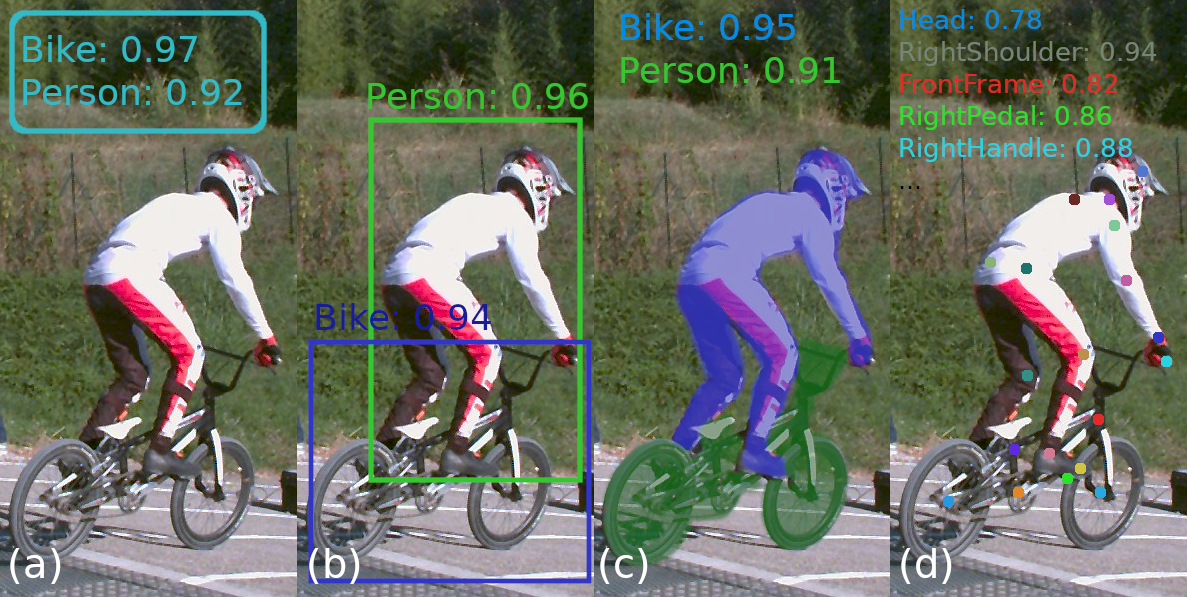
\includegraphics[width=\linewidth]{"../Chap2/Figures/Fig_classif_detec.png"}
	\caption{Mock examples of different types of image analysis. (a) Whole image classification, (b) Object detection and localization, (c) Instance segmentation and shape extraction, (d) Keypoint detection.}
	\label{fig_classif_detec}
\end{figure}

\subsection{Machine Learning Timeline and Principles}

Machine learning is a subset of artificial intelligence (AI.) As such, one can trace its origin back to the discovery of the natural neuron at the end of the 19th century, by Nobel Prize Ramón y Cajal \cite{Lopez2006}, followed half a century later by the first model of an artificial neuron \cite{Mcculloch1943}. A natural neuron is a simple learning unit, which collects the nervous influx sent by other neurons to its dendrites, and sends an action potential when the total influx weighted and summed in the soma overcomes a threshold value. This potential is then transmitted through the axon to the next neuron as a new influx. Similarly, an artificial neuron receives output vectors from previous neurons, weighs and sums them with a summation function, and transfers the resulting output vector to the next neurons if it reaches a certain threshold determined by an activation function (Figure~\ref{fig_neuron}a-b). 

The perceptron, invented in 1956 \cite{Rosenblatt1958}, represents the first practical application of an artificial neuron. It acts as a binary classifier which predicts class 1 if the neuron is fired, and class 0 otherwise. It automatically adjusts its weights by learning from previously labeled example data (see Algorithm~\ref{alg:perceptron} and Figure~\ref{fig_neuron}b). It could be used, for example, to predict whether an athlete is going to be "good" or not, given his force-velocity results on an ergometer test (see step-by-step \hyperlink{example1}{Example 1} and Figure~\ref{fig_perceptron}), and given enough example data. Needing previously labeled data makes it is a supervised classifier – we will not discuss unsupervised methods here. Of course, this example is oversimplified. Being good or not at a sports is a complex and multifactorial outcome, and two variables can't sum it up. However, the perceptron can take more than two variables as inputs (for example, force, velocity, and endurance), and it can also be generalized to multiclass classification with more than two outputs (for example, to differentiate between strong, explosive, and resistant type of athletes.)

Nevertheless, it often takes a lot of iterations over good quality training data for the perceptron to converge. Moreover, it does converge if and only if the data are linearly separable, i.e., if they can be separated with a straight line \cite{Novikoff1963} (see Figure~\ref{fig_linearly_sep}). Some fundamental problems such as the XOR gate can't be solved with a basic single layer Artificial Neural Network (ANN) \cite{Minsky1969}. This constituted one of the early setbacks for AI. Then, the high computational cost of these approaches, combined with the complexity of common-sense problems, hampered the trust in learning methods. Indeed, vision and language problems require enormous amounts of data, and can't be solved with a simple dictionary (for example, "the spirit is willing but the flesh is weak" becomes "the vodka is good but the meat is rotten" when translated back and forth from English to Russian.) Overinflated promises and expectations, followed by disappointment in academia and industries, led to cuts in funding, and eventually loss of skills in the 1970s: this is referred to as the first AI winter.

The AI field survived by focusing on specific problems, called expert systems. In the early 1980s, a new rise was triggered by massive funding such as the Japanese Fifth Generation Computer project, aiming to build a supercomputer that could solve any problem. Shortly after, multi-layer neural networks were made possible with the (re)discovery of backpropagation \cite{Rumelhart1986}, or more rigorously of weight adjustment thanks to the backpropagation of error gradient, from the last layer to the first one. As it is not the central subject of this thesis, the algorithm and early references will not be detailed here, but the interested reader can refer to \cite{Goodfellow2016}. This allowed for solving non-linearly separable problems, and for tackling real world issues (Figure~\ref{fig_neuron}c.). \cite{Cybenko1989} proved that one single intermediate layer is enough to solve any given classification problem, granted that this layer contains enough neurons (although sometimes too many to make it possible in practice.) On the other hand, kernel tricks were also rediscovered \cite{Aizerman1964,Hofmann2008}, and made non-neural networks such as support vector machines (SVMs) \cite{Boser1992} able to treat non-linearly separable data with much less training data, more optimally, and on a clearer mathematical ground (Figure~\ref{fig_linearly_sep}). However, again, unrealistic expectations were confronted with unplanned technical difficulties both on expert systems and on general intelligence projects. This led to a second AI winter in the 1990s. 


\begin{figure}[hbtp]
	\centering
	\def\svgwidth{1\columnwidth}
	\fontsize{10pt}{10pt}\selectfont
	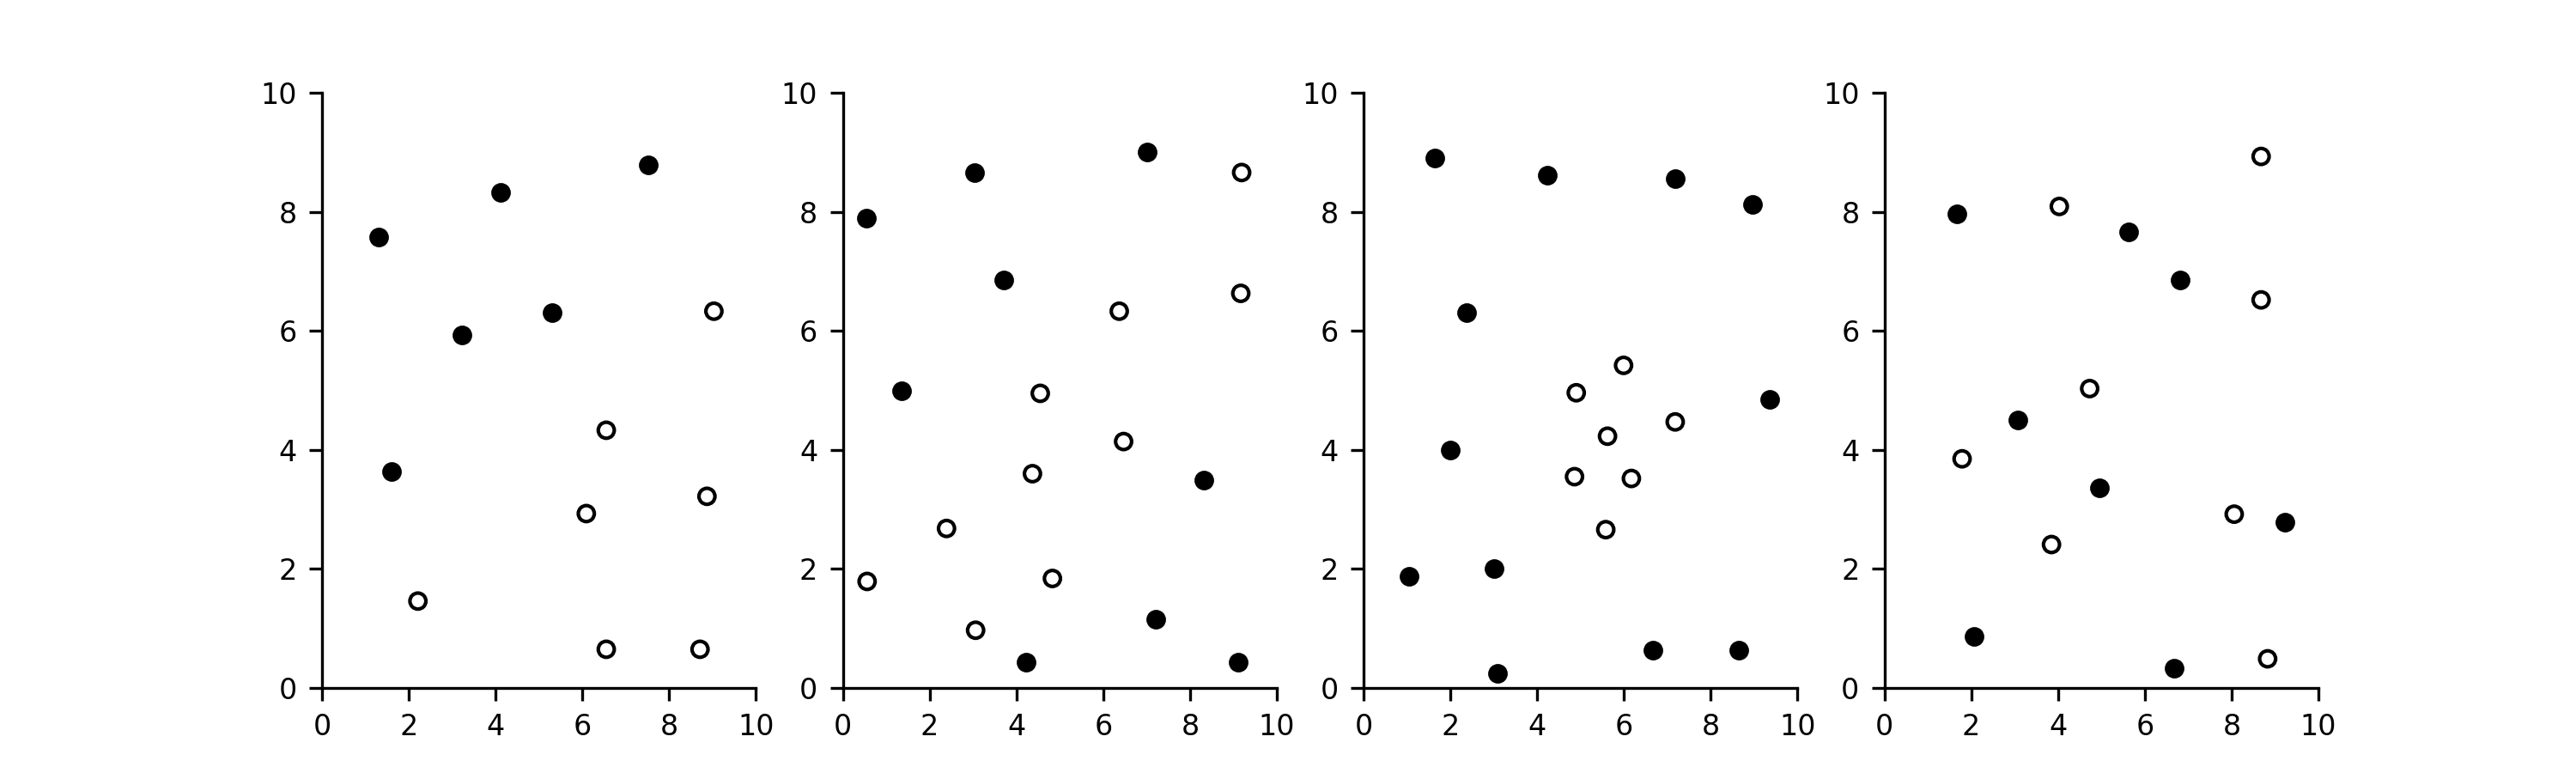
\includegraphics[width=1\linewidth]{"../Chap2/Figures/Fig_linearly_sep.png"}
	\caption{Single layer artificial neural networks such as the perceptron can only classify linearly separable data. (a) is linearly separable. (b) is not linearly separable. However, data are contained in an ellipse. The equation of an ellipse is of the form \(a \times x^2+b\times y^2=1\), so if we transform the feature variables into \(X=x^2\) and \(Y=y^2\), the data become linearly separable. (c) is equivalent to a fundamental XOR gate, and is not linearly separable, which was part of the reasons for the first AI winter. It can either be solved by combining several layers of artificial neurons, or by complex kernel tricks which map the data from the original space into a higher dimensional space where they become linearly separable. (d) is possibly not separable at all. AI: Artificial Intelligence. XOR: Exclusive OR.} 
	\label{fig_linearly_sep}
\end{figure}

\begin{figure}[!ht]
	\centering
	\def\svgwidth{1\columnwidth}
	\fontsize{10pt}{10pt}\selectfont
	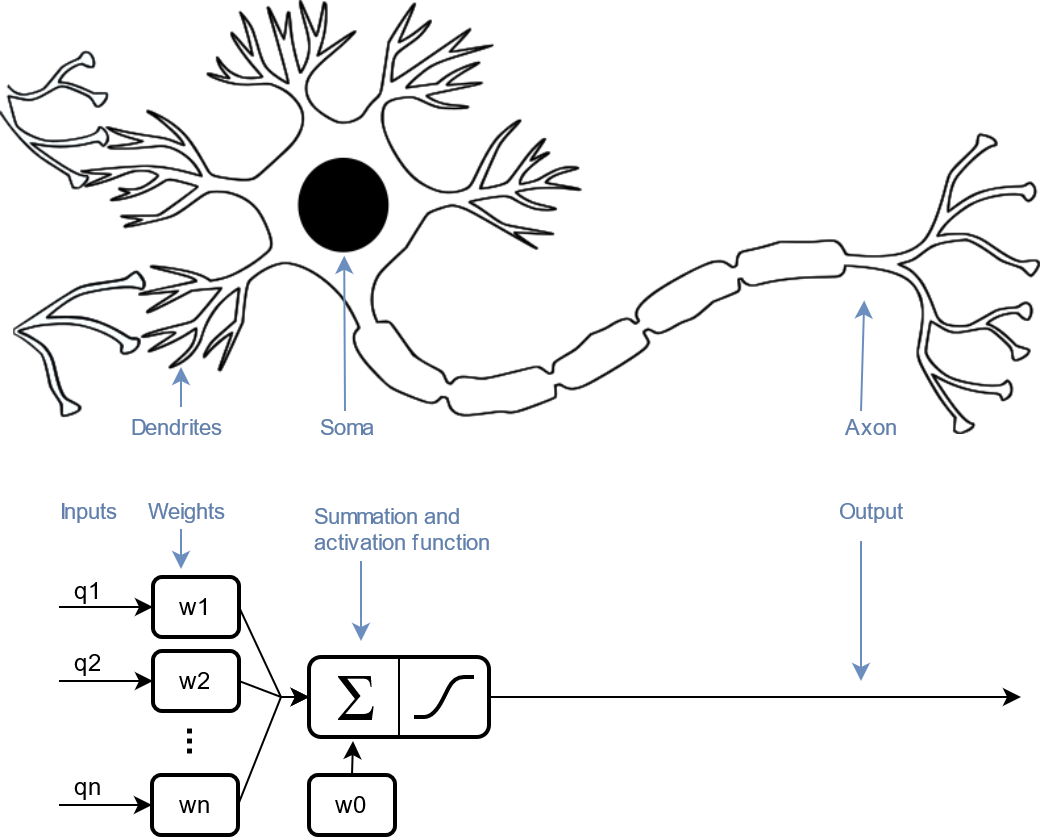
\includegraphics[width=0.95\linewidth]{"../Chap2/Figures/Fig_neuron.png"}
	\caption{The artificial neuron (b) has been modeled after the natural neuron (a). Inputs and weights act as the total nervous influx firing the dendrites. The collected values are summed, and a signal is activated if a threshold is overcome, as the soma does in a natural neuron. The output signal is conveyed the axon in a natural neuron. (b) In the case of a perceptron, the neuron adjusts its weights to minimize the error between the predicted and the expected output. It can be used as a classifier, which outputs class 1 or class 0 depending on the inputs. (c) A dense (fully connected) neural network with one intermediate layer and backpropagation can solve any non-linearly separable classification.}
	\label{fig_neuron}
\end{figure}

\clearpage
\begin{algorithm}[!ht]
  \caption{Perceptron}\label{alg:perceptron}
  \begin{algorithmic}[1]
    \STATEx Let \( \overrightarrow{X^0} \) be the input vector of a first instance of variables \( (1, x_1^0, \cdots x_M^0) \), \( \overrightarrow{W^0} \) the corresponding weights randomly initialized \( (w_0^0, w_1^0, \cdots w_M^0) \) with \(w_0^0\) a bias, and \(y^{0, pred}\) the output predicted binary class. 
    \STATE The summation function is computed: 
    \begin{equation}
        \overrightarrow{W^0} \cdot \overrightarrow{X^0} = \sum_{m \in [0,M]} w_m^0 x_m^0
    \end{equation}
    \STATE This result is processed by an activation function, which is a threshold in the case of the perceptron. It determines whether the neuron will be fired or not, i.e., whether one or the other class will be predicted. $y^{0,pred}$ = 1 corresponds to one class, and $y^{0,pred}$ = 0 to the other. 
    \begin{equation}
        y^{0,pred} = 
        \begin{cases}
            1 & \text{if} \ \overrightarrow{W^0} \cdot \overrightarrow{X^0} > \theta,\\
            0 & \text{otherwise}
        \end{cases}
    \end{equation}
    \STATE This prediction $y^{0,pred}$ is compared to the actual class $y^{0,expected}$. 
    \begin{equation}
        \epsilon^0 = y^{0,expected} - y^{0,pred}
    \end{equation}
    \STATE Then weights are updated: 
    \begin{equation}
        \overrightarrow{W^1} = \overrightarrow{W^0} + \eta \ \epsilon^0 \ \overrightarrow{X^0}
    \end{equation}
    \STATEx with $\eta$ the learning rate $\in$ [0,1]. Note that if the class is correctly predicted, then $\epsilon^0=0$ and weights are not adjusted.   
  %   \STATEx \textit{In Adaline, weights are adjusted early and in a continuous way, before being processed by the activation function: \(\epsilon^0 = \frac{\partial \frac{1}{2}(y^{0,expected} - \overrightarrow{W^0} \cdot \overrightarrow{X^0})^2}{\partial \overrightarrow{W^0}}= y^{0,expected} - \overrightarrow{W^0} \cdot \overrightarrow{X^0}\)}.
  \STATE The algorithm is repeated with another example $\overrightarrow{X^1}$, and so on until it has gone through the whole batch of the training set. If weights still need to be updated, one can go over it again, for a determined number of epochs or until the average error is under a given value. Then the perceptron is considered trained, and ready to correctly predict a class $y$ with the retained weights.
  %   \algstore{alg1}
  \end{algorithmic}
\end{algorithm}

% \begin{algorithm}
%       \begin{algorithmic}[1]
%         \algrestore{alg1}
%         \STATE bla
%       \end{algorithmic}
% \end{algorithm}

\begin{tcolorbox}[nofloat, colback=white,colframe=black, colbacktitle=white, coltitle=black, breakable, title=\textbf{Example 1} Athlete classification with a perceptron, label=example1]
      \phantomsection\hypertarget{example1}
      N.B. The code for running this example is available on the thesis repository \url{https://github.com/davidpagnon/These_David_Pagnon/blob/main/Thesis/Chap2/perceptron.py}.
      \tcblower
      Let's consider force-velocity test results as an input
      \setlength{\belowdisplayskip}{0pt} \setlength{\belowdisplayshortskip}{0pt}
      \setlength{\abovedisplayskip}{0pt} \setlength{\abovedisplayshortskip}{0pt}
      \begin{flalign*}
      \overrightarrow{X} = (1, velocity \ (m/s), force \ (hN) ), && 
      \end{flalign*}
      and the classification of an athlete as "skilled" or "unskilled" as an output
      \(y = 1 \ or \ 0. \)\newline
      A batch of training data, i.e., example data the perceptron will learn from, could be: 
      \[ \bigl\{(\overrightarrow{X^i}, y^{i, expected})\bigr\}_{i\in [0,4]}
      = \bigl\{\bigl((1, 1, 5), 1\bigr),
      \bigl((1, 2, 3), 0\bigr),
      \bigl((1, 7, 1), 1\bigr),
      \bigl((1, 4, 1), 0\bigr),
      \bigl((1, 5, 4), 1\bigr)\bigr\}. \]
      
      Let's randomly initialize weights at \(\overrightarrow{W^0} =  (-9, 1, 3) \), take a threshold $\theta$=0.1, and a learning rate $\eta$ = 0.3.\newline
            
      \textbf{The first instance} of the training set gives: 
      \begin{flalign*}
      \overrightarrow{W^0} \cdot \overrightarrow{X^0} = \sum\nolimits_{m \in [0,2]} w_m^0 x^0_m = -9 \times 1+ 1 \times 1 + 3 \times 5 =7.&&
      \end{flalign*}
      Now \(\overrightarrow{W^0} \cdot \overrightarrow{X^0} = 7 > \theta = 0.1\), so $y^{0, pred} = 1$.\newline
      \(y^{0, expected} = 1 = y^{0, pred} \), so the prediction is true and weights don't need to be updated. \newline
      As a consequence, \(\overrightarrow{W^1} = \overrightarrow{W^0} = (-9, 1, 3).\)\newline
      
      \textbf{The second instance} gives \(\overrightarrow{W^1} \cdot \overrightarrow{X^1} = (-9, 1, 3) \cdot (1,2,3) = 2 > \theta = 0.1\), so $y^{1, pred} = 1$. \newline
      But \(y^{1, expected} = 0 \neq y^{1, pred} = 1\), so weights need to be updated.\newline
      The error is \(\epsilon^1 = y^{1,expected} - y^{1,pred} = 0-1 = -1\).\newline
      As a consequence, \(\overrightarrow{W^2} = \overrightarrow{W^1} + \eta \ \epsilon^1 \ \overrightarrow{X^1} = (-9, 1, 3)  + 0.1 \times (-1) \times (1,2,3) = (-9.3,0.4,2.1).\)\newline
      
      \textbf{Third instance}: \(\overrightarrow{W^2} \cdot \overrightarrow{X^2} = (-9.3,0.4,2.1) \cdot (1,7,1) = 3-4.4 < 0.1\), so $y^{2, pred} = 0$. \newline
      \(y^{2, expected} = 1 \neq y^{2, pred} = 0\), so weights need to be updated.\newline 
      \(\epsilon^2 = y^{2,expected} - y^{2,pred} = 1\).\newline
      \(\overrightarrow{W^3} = \overrightarrow{W^2} + \eta \ \epsilon^2 \ \overrightarrow{X^2} = (-9.3,0.4,2.1) + 0.1 \times 1 \times (1,7,1) = (-9,2.5,2.4).\)\newline
      
      \textbf{Fourth instance}: \(\overrightarrow{W^3} \cdot \overrightarrow{X^3} = (-9,2.5,2.4) \cdot (1,4,1) = 3.4 > 0.1\), so $y^{3, pred} = 1$. \newline
      \(y^{3, expected} = 0 \neq y^{3, pred} = 1\), so weights need to be updated.\newline
      \(\epsilon^3 = y^{3,expected} - y^{3,pred} = -1\).\newline
      \(\overrightarrow{W^4} = \overrightarrow{W^3} + \eta \ \epsilon^3 \ \overrightarrow{X^3} = (-9,2.5,2.4) + 0.1 \times (-1) \times (1,4,1) = (-9.3,1.3,2.1).\)\newline
      
      \textbf{Fifth instance}: \(\overrightarrow{W^4} \cdot \overrightarrow{X^4} = (-9.3,1.3,2.1) \cdot (1, 5, 4) = 17.6 > 8\), so $y^{4, pred} = 1$. \newline
      \(y^{4, expected} = 1 = y^{4, pred} = 1\), so weights don't need to be updated.\newline
      \(\overrightarrow{W^5} = \overrightarrow{W^4} = (-9.3,1.3,2.1) (Figure~\ref{fig_perceptron}). \)\newline

      \textbf{Next instances}: Once we have gone over the batch of training data, if the average error is below a given value, we can assume that the perceptron is trained. If not, we can use the next batch to pursue training. If it still didn't converge after all batches, we can iterate over all training data again, for a given number of times. If results are still not satisfying, either the data are not linearly separable, or the training sample is not large enough or of good enough quality. In our case, it seems like our example data have allowed us to correctly separate skilled and unskilled athletes based on their force and velocity test results (Figure~\ref{fig_perceptron}).

      {
      \begin{center}
      \def\svgwidth{1\columnwidth}
      \fontsize{10pt}{10pt}\selectfont
      \centerline{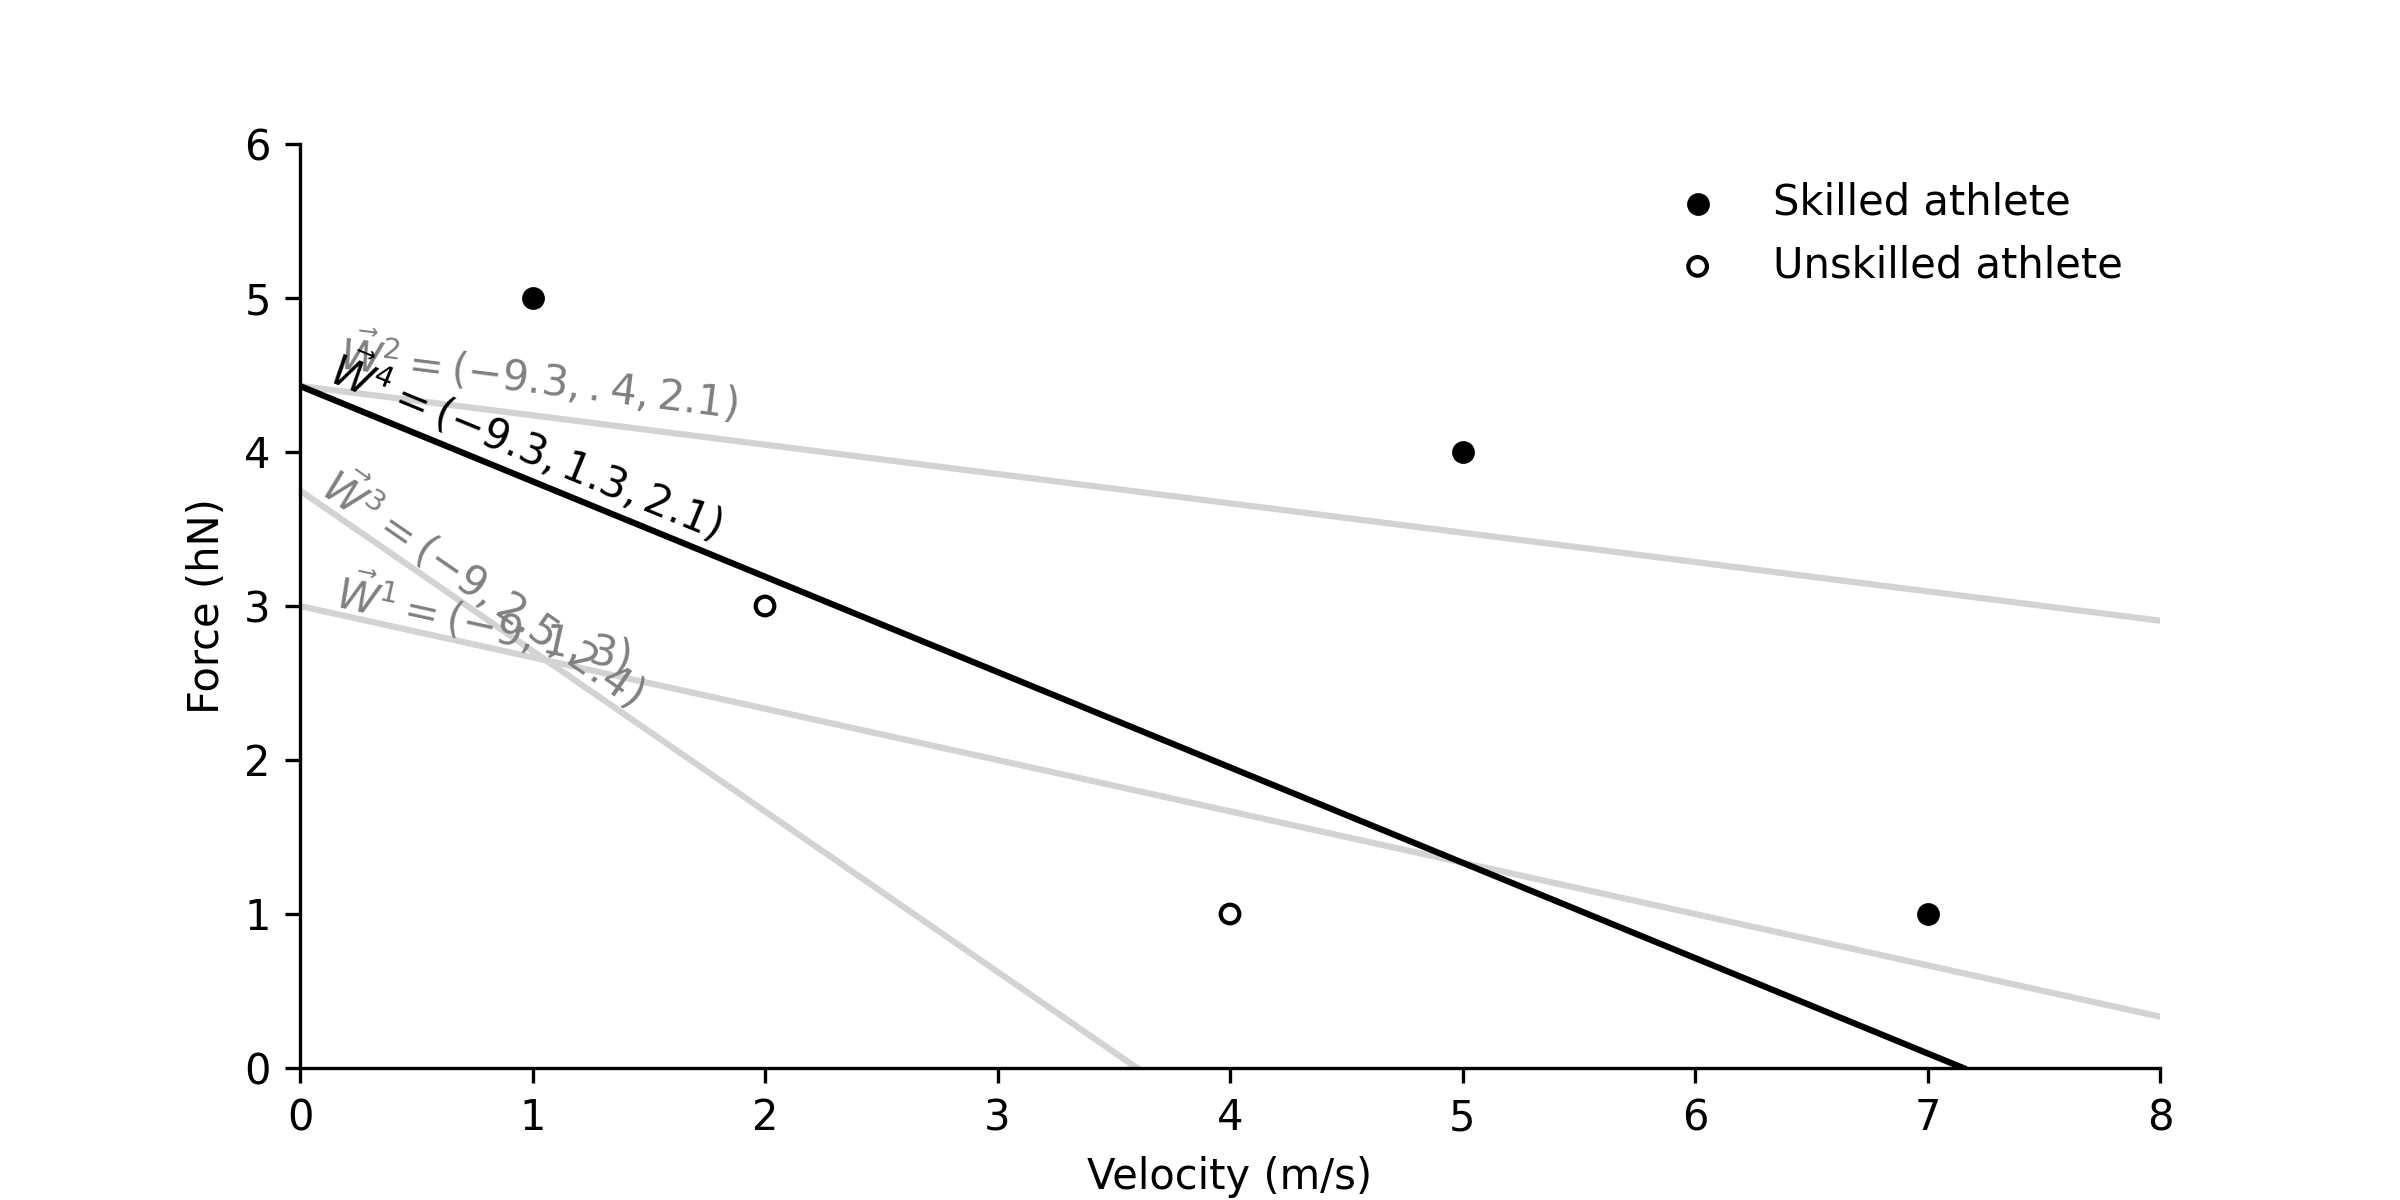
\includegraphics[width=0.9\linewidth]{"../Chap2/Figures/Fig_perceptron.png"}}
      \captionof{figure}{Classification of athletes as "skilled" (black dot) or "unskilled" (circle) according to their Force-Velocity results. Weights are adjusted (grey lines), until the perceptron classifies athletes correctly (black line.)}
      \label{fig_perceptron}
      \end{center}
      }
\end{tcolorbox}

\newpage

From the end of the 1990s, there has been no theoretical breakthrough in AI, but larger databases have become available with the advent of the Internet, and greater computational power has become accessible, especially thanks to groundbreaking progress in Graphics Processing Units (GPUs), which made heavy parallel computing available to the wider audience. As a consequence, more layers could be used in neural networks, which progressively set off the onset of deep learning. Finally, complex "common-sense" problems, such as natural language processing or image recognition, could be treated with some success \cite{Baral2018}.

One particular type of deep learning algorithms is the convolutional neural network (CNN), which is particularly suited for image recognition. It was first used for classifying handwritten and low-resolution digits \cite{LeCun1998}, and then applied to more complex images as greater computing resources became available \cite{Krizhevsky2017}. Nowadays, CNNs have sometimes surpassed humans at image classification \cite{Cireşan2012, Lu2015}. A convolution layer consists of a series of filters that slide across the image, each of them outputting a result close to 0 or to 1, depending on how well it can be overlaid on each image area. In the same way as with a simple artificial neuron, each of these filters can be seen as a weight vector \(\overrightarrow{W}\), and each image area as an input vector \(\overrightarrow{X}\). The filters of the first convolution layer are simple patterns such as lines, but then they become circles and corners, until the last layers, when they have developed into complex features corresponding to whole object parts. Once a filter has covered the whole image, it forms a feature map, which will then be downsampled by a pooling layer in order to save computing resources. All the feature maps produced by each filter are processed by a determined number of other convolution layers, and then flattened into a 1D vector. This 1D vector is processed by a few dense layers (dense layers are fully connected, i.e., all outputs are produced by a weighted sum of each input), and lastly a softmax layer computes a probability for the image to correspond to each available class. If the CNN is correctly trained, the class with highest probability corresponds to the correct one: for example, if the image displays a BMX start, the probability for the bike class will be the highest (Figure~\ref{fig_cnn}). 

However, results will not be good until a lot of iterations are done on a lot of data. Indeed, filters at each layer are randomly initialized, and then refined with backpropagation in order to predict all classes as best as possible. One of the risks is overfitting, i.e., to excessively adapt to the training data and to fail to generalize to new data. This is dealt with by cross-validation, i.e., the separation between training and test data, by regularization methods such as radomization, batch normalization and dropout, and by data augmentation, e.g., image rotations, crops, color distortion, noise addition, etc. \cite{Hawkins2004,Chicco2017} (Figure~\ref{fig_xkcd}). An enormous amount of data is also needed to correctly train the CNN, which makes it complicated when unusual classes need to be recognized (for example, a climbing hold, a BMX starting gate, a medial malleolus on the ankle, etc.) Fortunately, one can consider that a CNN trained on a massive dataset, such as ImageNet and its 14 million annotated images \cite{Deng2009}, has learned to recognize most features that can be found in any image. One can take the learned filters of its convolutional layers as is, use them as a feature extractor (sometimes called backbone), and just fine-tune the last dense layers to recognize new classes. It will be much less computationally expensive to train, and will need much fewer data: about a hundred images, instead of thousands. This is called transfer learning \cite{Pan2009}.

Now, classification of a whole image is not sufficient in sports motion analysis. One needs to detect where an object or a person is, and ideally to localize more precise features such as joint centers so as to estimate the person's pose. 

\clearpage
\begin{figure}[hbtp]
	\centering
	\def\svgwidth{1\columnwidth}
	\fontsize{10pt}{10pt}\selectfont
	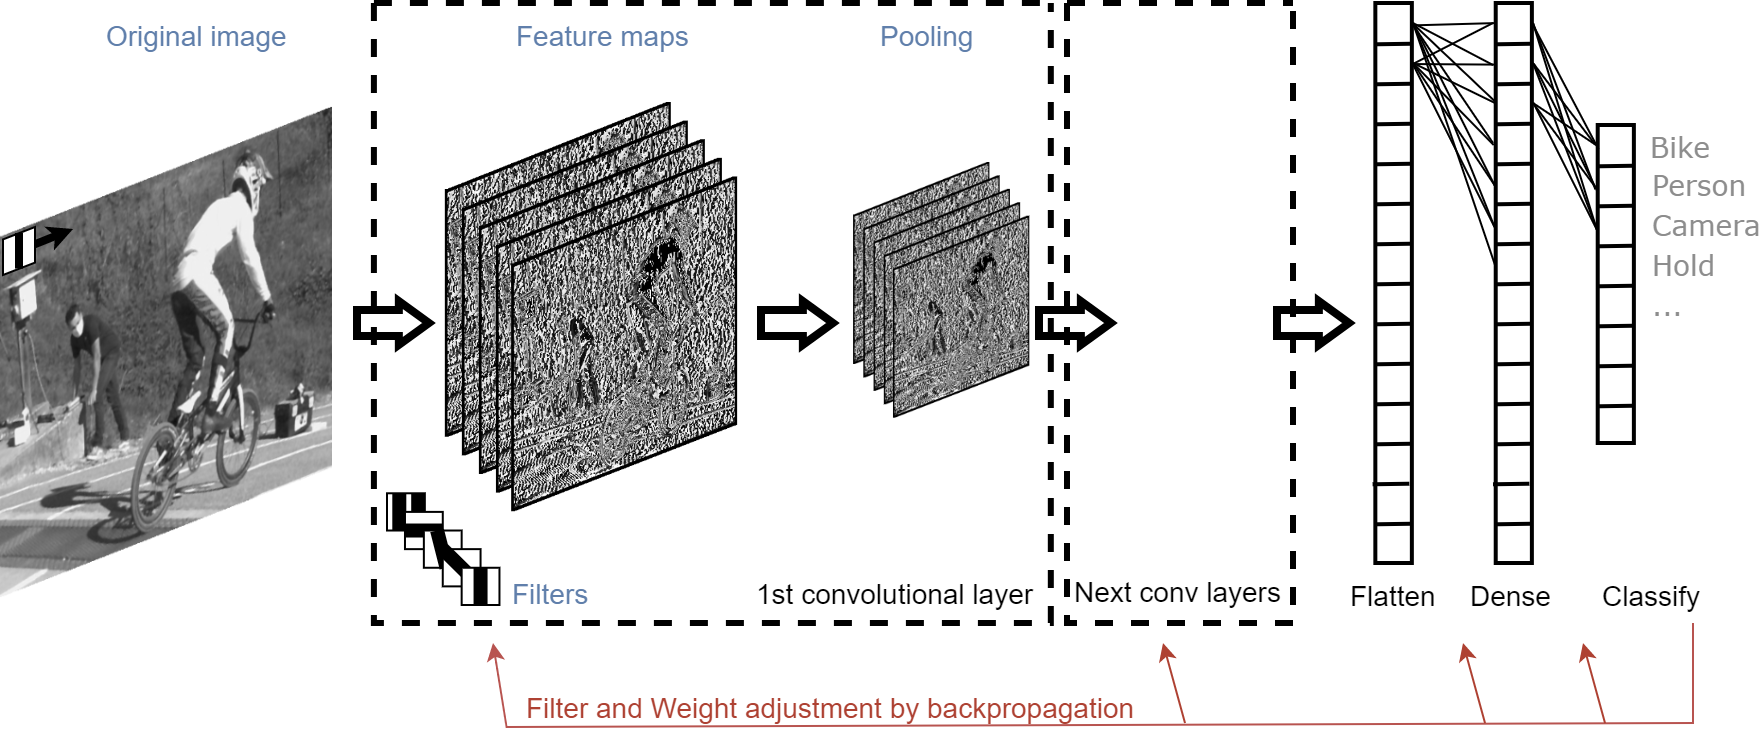
\includegraphics[width=1\linewidth]{"../Chap2/Figures/Fig_CNN.png"}
	\caption{A simplified convolutional neural network (CNN.) A convolutional layer consists of a series of filters running across the input image, and producing feature maps, which are then downsampled by pooling. Filters become more and more elaborated along layers, and produce feature maps which look like whole object parts. Filters and weights are randomly initialized at first, and then are adjusted by backpropagation. After the convolutional layers, the feature maps are flattened to produce a 1D vector, which is then processed by dense layers, and finally a softmax layer computes a probability for the image to correspond to each available class.} 
	\label{fig_cnn}
\end{figure}

\begin{figure}[hbtp]
	\centering
	\def\svgwidth{1\columnwidth}
	\fontsize{10pt}{10pt}\selectfont
	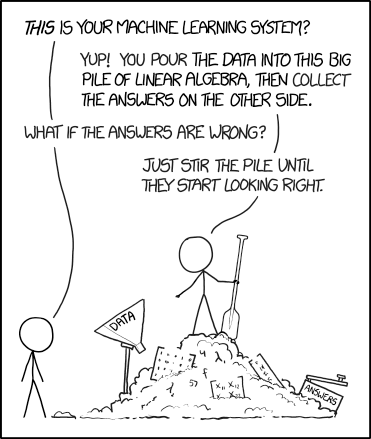
\includegraphics[width=0.4\linewidth]{"../Chap2/Figures/Fig_XKCD.png"}
	\caption{The amazingly rigourous world of machine learning. \href{https://xkcd.com/1838/}{XKCD} .} 
	\label{fig_xkcd}
\end{figure}


\subsection{Machine Learning for 2D Pose Estimation}\label{sec:Machine learning for 2D pose detection}

Older methods for object detection used to run a sliding and pyramidal window across the image, and then to apply a non-neural classifier on each window, such as an SVM on carefully handcrafted histogram of oriented gradients descriptors (HOG) \cite{Dalal2005}. They then had to be followed by non-maximum suppression, in order to select one bounding box over many overlapping ones. As the classifier is run on each window iteration like if they were independent images, these methods were very computationally intensive, and in the same time not very robust nor accurate. 

\clearpage
More modern approaches are based on CNNs, and as such, they involve a preliminary step: extracting the last layer of a pre-trained neural network such as ImageNet, in order to make it able to classify the objects of interest. One of the precursors, R-CNN (Regions with CNN features) \cite{Girshick2014}, first looks for a lesser amount of regions of interest (ROIs) by selective search, instead of with a sliding window. Selective search is an algorithm which segments image based on pixel intensities, without any learning involved \cite{Uijlings2013}. Then three learning models are used: one CNN for extracting features from each ROI, an SVM for classifying each ROI, and a regression model for adjusting bounding boxes. It takes about 45 seconds to process a single image on benchmarks. Fast R-CNN \cite{Girshick2015} uses one single network for all steps, and switches the first two: it first extracts features from the whole image, and only then uses selective search to find ROIs on the resulting feature map, and finally classifies the ROIs and tightens the bounding boxes. It is much faster and takes about 2 seconds per image. A last incrementation on this basis is Faster R-CNN \cite{Ren2015}, which works similarly to the latter, but finds ROIs with a neural network instead of with selective search, which is very time-consuming. This allows for predicting an "objectness" score on each ROI, and for fitting the bounding boxes directly, and thus on avoiding the last regression step. It is even faster, and takes about 0.2 seconds per image. YOLO (standing for You Only Look Once) \cite{Redmon2016} proposes another approach, and does not separate the steps of finding ROIs with classification. It divides the image into regions, and predicts both classes and bounding boxes for each region. For example, if there is a shoulder in a region, it will predict a "person" class, and a larger box in which this person is likely to fit. YOLO takes about 0.02 seconds per image (45 fps), and is thus able to run real time. However, it is not as accurate as the previous methods, especially on smaller objects. This being said, new versions are very frequently released (although not by the same authors), and the current YOLOv7 \cite{Wang2022b} is both faster and more accurate than all previous approaches as it entirely reviews the whole network architecture to deal with all observed bottlenecks.

But again, in order to perform joint kinematics, one cannot just detect whole objects: precise keypoints need to be localized. Mask R-CNN \cite{He2017}, and the more recent Detectron2 \cite{Wu2019}, still predict the bounding boxes and their class like Faster R-CNN does, but they also add a small overhead in parallel, which predicts the shapes of masks overlaying the object in a pixel-to-pixel manner. Keypoints can be seen as a very small mask, and Mask R-CNN can also detect them in order to predict human pose estimation. In the next paragraph, only multi-person pose estimation models will be considered. Datasets, evaluation metrics, and comparison of results won't be detailed: see \cite{Topham2021} for a comprehensive overview.

Two main approaches for multi-person 2D pose estimation coexist. The "top-down" one first detects bounding boxes around persons, and then finds keypoints inside each box. In the area of object detection methods, it is analogous to region-proposed methods such as the R-CNN suite, which proposes ROIs and then finds and classifies objects. Conversely, the "bottom-up" approach first finds keypoints, and then groups them into persons. It is analogous to the single-shot object detection methods such as the YOLO suite, which first finds small details, and then predicts full-size objects. These approaches are nowadays almost as fast as the top-down ones, and their inference time does not increase with the number of persons detected. 

Mask R-CNN belongs to the top-down kind, as well as AlphaPose \cite{Fang2017}, which mostly differentiates from the latter by using a network predicting higher quality bounding boxes from inaccurate ones, in order to facilitate the task of the joint regressor. On the opposite, DeepCut and DeeperCut \cite{Pishchulin2016,Insafutdinov2016}, as well as DeepLabCut \cite{Mathis2018,Lauer2022} upon which it is built, are bottom-up approaches. They find a large number of keypoint candidates, label them as hand, head, etc., and then select the best candidates and separate them into persons. Since they calculate every possible association between keypoints, this is very slow. OpenPose \cite{Cao2019} uses a network which jointly predicts keypoint locations, and the connections between them (i.e., it also predicts limbs, which define a skeleton), and is much faster while still being accurate. OpenPifPaf \cite{Kreiss2021} adds to it both temporal consistency across frames, and an intensity map for each keypoint instead of punctual locations (i.e., a further keypoint will have a lower intensity). This allows for better accuracy in low-resolution regime and in occluded images. YOLOv7 supports keypoint detection by integrating YOLO-Pose \cite{Maji2022}, and claims to be faster and more accurate than all other state-of-the-art methods. It brings together top-down and bottom-up approaches, and uses a single network predicting both bounding boxes and their corresponding poses. SLEAP \cite{Pereira2022}, which is built for training animal pose estimation models, implements both top-down and bottom-up approaches. In this context, top-down approaches are slightly more accurate, and considerably faster as long as few animals are in the scene.

\begin{figure}[hbtp]
	\centering
	\def\svgwidth{1\columnwidth}
	\fontsize{10pt}{10pt}\selectfont
	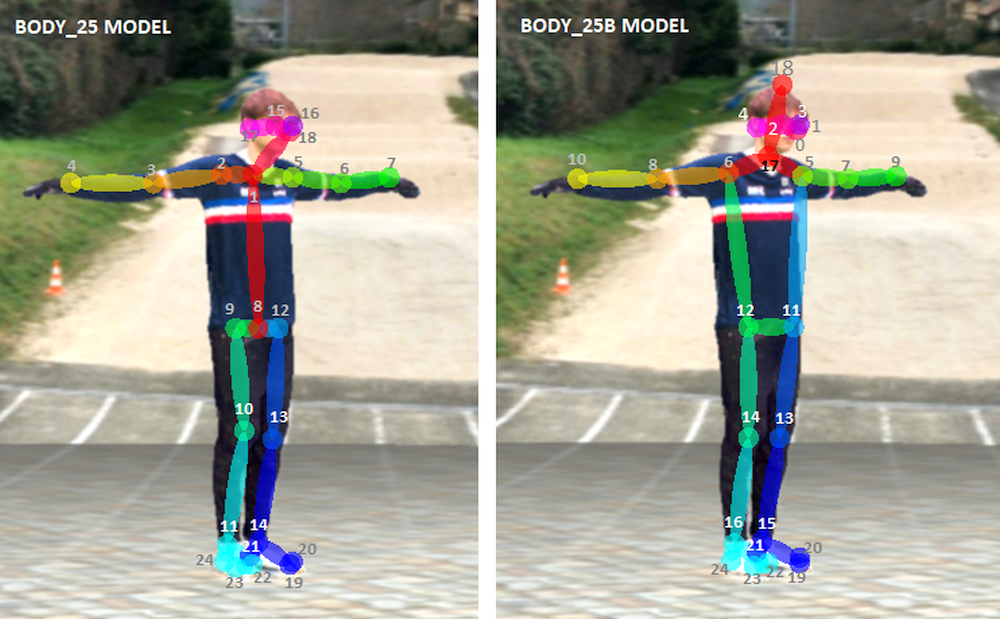
\includegraphics[width=1\linewidth]{"../Chap2/Figures/Fig_body25b.png"}
	\caption{The body\_25b OpenPose model is more accurate than the default body\_25 one. As an example, the left knee is slightly misplaced on the default model. Keypoint definition and order also differ between both models.} 
	\label{fig_body25b}
\end{figure}

Like all previously presented methods, OpenPose has been trained on the COCO dataset \cite{Lin2014}. However, OpenPose body\_25 standard model also provides foot keypoints, which are often primordial in sports motion analysis. To do so, 6 more keypoints have been labeled for the feet on the COCO dataset before training. OpenPose also supports the single-network whole-body pose estimation network body\_135 \cite{Hidalgo2019}, which has been trained in the same time on COCO+foot,  MPII \cite{Andriluka2014}, and on Total Capture \cite{Xiang2019} in order to provide hand, face, feet, and body keypoints in one single network. The body\_135 model is slow and requires high capacity hardware, however a submodel of it is body\_25b, which provides body and foot keypoints as body\_25 does, and in addition decreases the number of false positives without hampering speed. Its keypoint definition differs slightly to the default model's (Figure~\ref{fig_body25b}): it adds the MPII head and neck keypoints, and removes the artificially created neck and middle hip points of the body\_25 model (which are simply the middle point of the shoulders and the hips). In a similar way, AlphaPose provides full-body models, either trained on the Halpe dataset \cite{Li2020}, or on the COCO-WholeBody one \cite{Xu2022}. Note that BlazePose \cite{Bazarevsky2020}, trained on the GHUM dataset \cite{Xu2020b}, also provides hand and feet keypoints, but since it is a single-person pose estimation model, the architecture is different and will not be addressed here. Indeed, this is rarely suitable in sports conditions, where people are usually present in the background. 


\FloatBarrier
\section{From 2D to 3D Pose Estimation}\label{sec:3D reconstruction}
\label{ch:2.2}

Once the pose of an athlete is correctly detected, the next step is to obtain their 3D pose. While some approaches strive to infer 3D pose from a monocular video source, they are generally not considered sufficiently accurate, especially when body parts are occluded. It is, then, important to use several cameras, and to fuse their 2D pose estimation results to obtain more reliable 3D coordinates.


\subsection{Pinhole Camera Model}\label{subsec:Pinhole model}

\subsubsection{History}

If it passes through a small enough hole, the light emitted from a point can be seen as a fine ray rather than a large beam. Then, when all the rays from the object go through, they do not overlap, and actually recreate an inverted image of it, instead of a blurry spot of light. If the hole gives entrance to a dark enough room, and if a light-colored sheet is positioned close enough to the hole, one can observe the projection of a dim, but distinct image of the object. This is the principle of the camera obscura, or pinhole camera, which might have been discovered as early as in the paleolithic era, as cave paintings seem to suggest. The concept was later used as a drawing aid in the $17^{th}$ century by some artists, probably such as Vermeer or Canaletto \cite{Steadman2001} (Figure~\ref{fig_camobscura}). In order to let more light in and to avoid diffraction issues, they increased the apperture of the hole and inserted in a convex lens, at the expense of a shorter depth of field and of some image distortion (Figure~\ref{fig_pinholelens}). Then, if instead of a sheet, a light-sensitive film is placed, the image is progressively printed, after enough light has struck it. This is how photography was invented in the $19^{th}$ century, by the French inventors Niépce, and then Daguerre \cite{Marignier1999}.

\begin{figure}[hbtp]
	\centering
	\def\svgwidth{\columnwidth}
	\fontsize{10pt}{10pt}\selectfont
	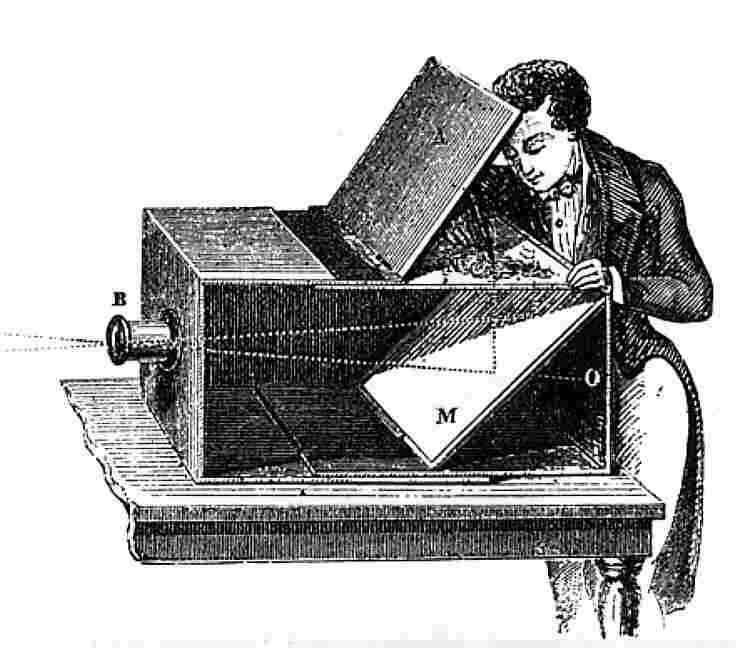
\includegraphics[width=0.8\linewidth]{"../Chap2/Figures/Camera_Obscura.jpg"}
	\caption{A camera obscura used as a drawing aid, which uses a lens rather than a pinhole (unknown author). } 
	\label{fig_camobscura}
\end{figure}

\begin{textblock*}{10cm}(13.2cm,22.45cm) % {block width} (coords left,top) 
  \begin{turn}{45} 
        \scriptsize \emojiegg
        \tiny 5. Merci aux gens de l'église ! 
        \scriptsize \emojichurch
  \end{turn}
\end{textblock*}

\begin{figure}[hbtp]
	\centering
	\def\svgwidth{\columnwidth}
	\fontsize{10pt}{10pt}\selectfont
	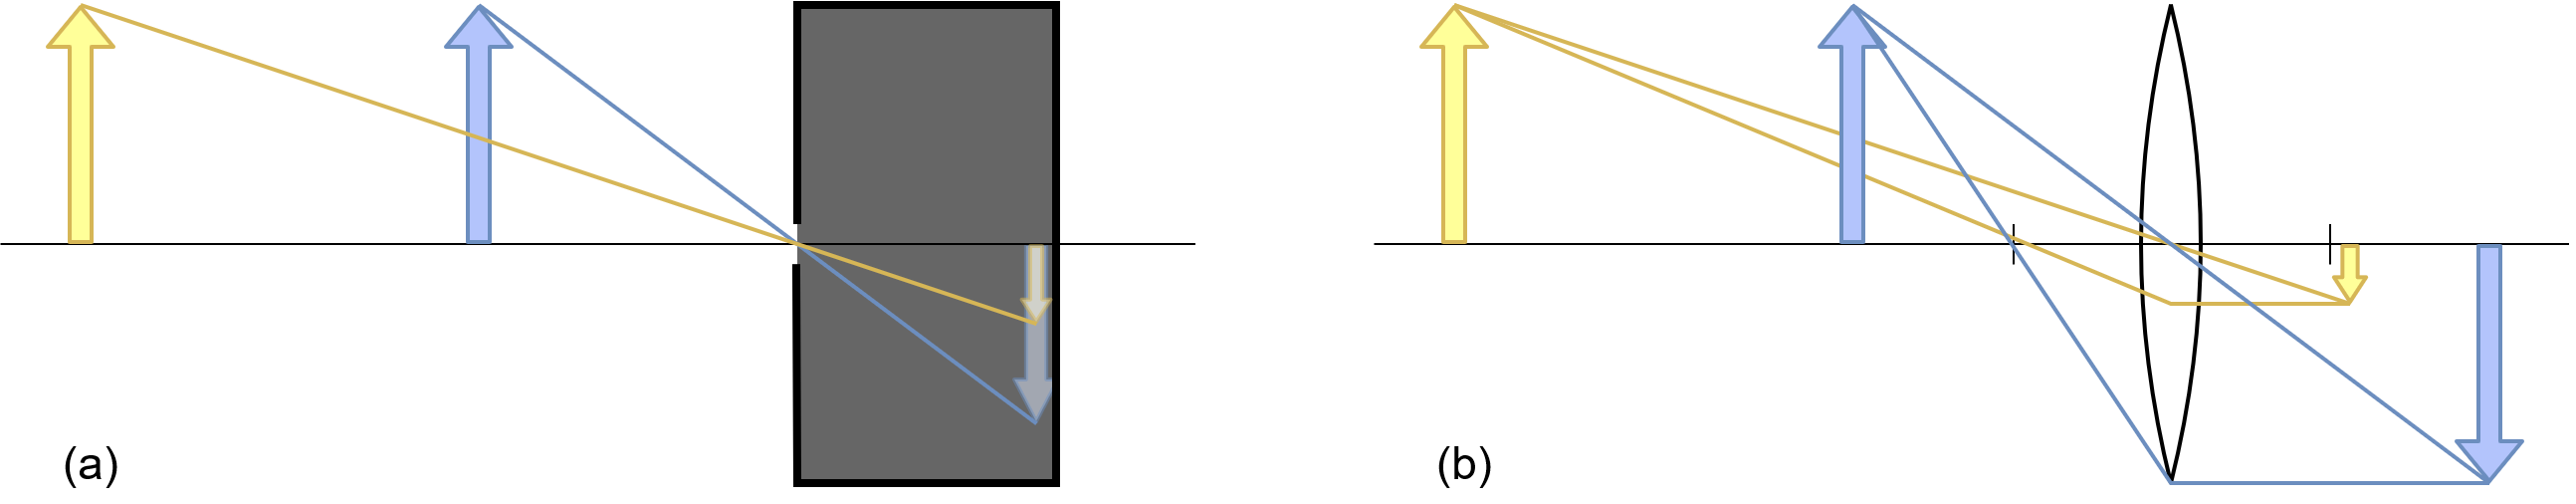
\includegraphics[width=1\linewidth]{"../Chap2/Figures/Pinhole_Lens.png"}
	\caption{(a) A pinhole camera does not need to be focused, because in theory, only one single ray per object point will pass through the apperture--which incidentally makes the image dimmer. (b) On the contrary, more light rays can pass through a lens, which makes the projected image clearer--but incidentally, it introduces a finite depth of field, as the image is focused on a different plane depending on the object distance to the lens.} 
	\label{fig_pinholelens}
\end{figure}


\subsubsection{Thin Lens}

When an object of size \(X_O\) (O standing for object) is projected from a distance \(Z_O\) through a thin convex lens of focal length \(f\), it is in focus at a specific distance \(z\). In this case, let the image size be \(x\). Assuming that the lens is thin, and that the object is close to the optical axis(i.e., that paraxial conditions are satisfied), Thales' theorem gives (Figure~\ref{fig_thinlens}):
\begin{equation}
  \begin{cases}
  &\frac{x}{X_O} = \frac{z}{Z_O} \text{ (dashed triangles)},\\
  &\frac{x}{X_O} = \frac{z-f}{f} \text{ (dotted triangles)},
  \end{cases}
\end{equation}

Which leads to the thin lens formula, discovered by Descartes in the $17^{th}$ century:
\begin{equation}
    \frac{1}{Z_O} = \frac{1}{f} - \frac{1}{z}
\end{equation}

\begin{figure}[hbtp]
	\centering
	\def\svgwidth{\columnwidth}
	\fontsize{10pt}{10pt}\selectfont
	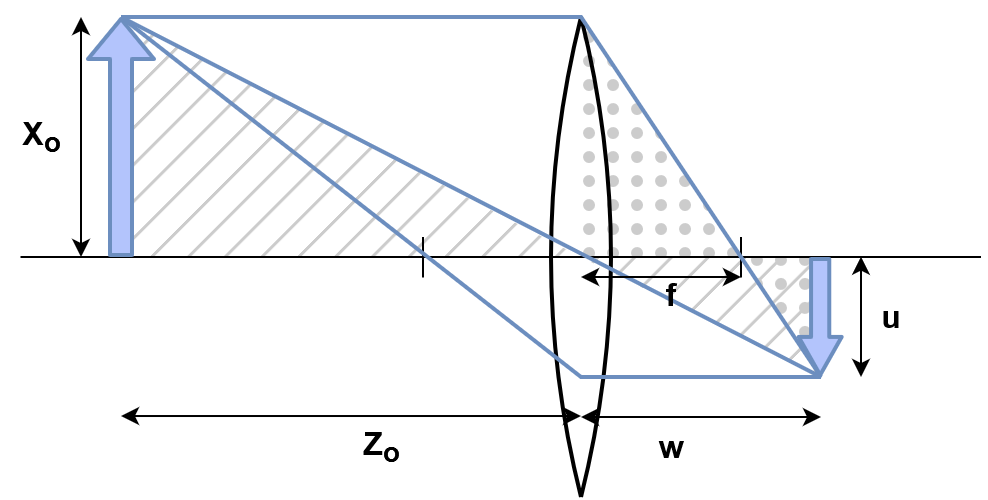
\includegraphics[width=0.5\linewidth]{"../Chap2/Figures/Thin_Lens.png"}
	\caption{Thales' theorem leads to the thin lens equation. \(X_O\) is the object of size, and \(Z_O\) its distance to the lens; \(x\) is the image size, and \(z\) its distance to the lens; and\(f\) is the focal length \(f\).} 
	\label{fig_thinlens}
\end{figure}

\subsubsection{Basic Pinhole Model}

According to the thin lens formula, in the specific case where the object is at a distance \(Z_O\) much larger than the focal length \(f\), one can approximate that the image is into focus at a distance \(z\) equal to the focal length. 
\begin{equation}
    z=f
\end{equation}

This is generally true in motion capture, for which the camera lens is usually focused to infinity, i.e., it looks at objects at least 100 times as far as the focal length. In this case, the Thales theorem gives the relation:
\begin{equation}
  x=\frac{f\times X_O}{Z_O}
\end{equation}

This model is called the basic pinhole camera model \cite{Zhang2000,Hartley2003,Tomasi2017}. This is strictly speaking improper, since a pinhole camera does not have any focal length. For the sake of simplification and since it does make a difference in practice, the image plane is usually represented upside-up and on the same side as the object (Figure~\ref{fig_cameralens}). 

\begin{figure}[hbtp]
	\centering
	\def\svgwidth{\columnwidth}
	\fontsize{10pt}{10pt}\selectfont
	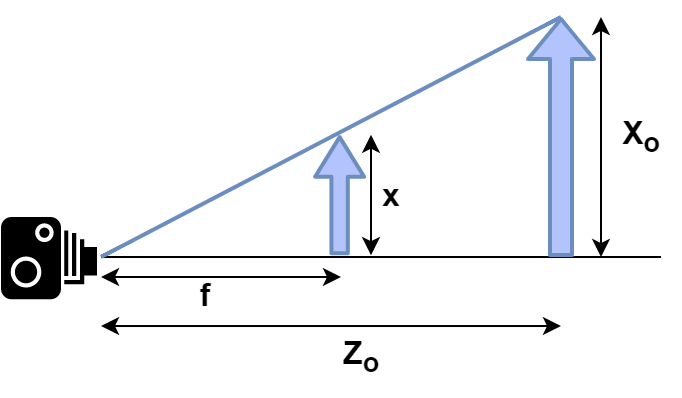
\includegraphics[width=0.5\linewidth]{"../Chap2/Figures/Camera_Lens.png"}
	\caption{The simplified pinhole camera model.} 
	\label{fig_cameralens}
\end{figure}


\FloatBarrier
\subsubsection{3D Pinhole Model in Camera Coordinate System}

In 3 dimensions, the object can be represented in the camera coordinate system $(X_C, Y_C, Z_C)$, with $Y_C$ pointing downwards, and $Z_C$ facing toward the object (Figure~\ref{fig_camera3d}). The relation becomes:
\begin{equation}
  \begin{cases}
  &x=\frac{f\times X_C}{Z_C},\\
  &y=\frac{f\times Y_C}{Z_C},
  \end{cases}
\end{equation}

Which can be written as:
\begin{equation}
  Z_C \times \begin{pmatrix}x\\y\end{pmatrix} 
  = \begin{pmatrix}f & 0 \\0 & f\end{pmatrix}\begin{pmatrix}X_C\\Y_C\end{pmatrix}
\end{equation}

% In the camera frame of reference instead of the object one, $X_C = X_O$, $Y_C = -Y_O$, and $Z_C = -Z_O$: 
% \begin{equation}
%   \begin{aligned}
%   &x=-\frac{f\times X_C}{Z_C},\\
%   &y=+\frac{f\times Y_C}{Z_C},
%   \end{aligned}
% \end{equation}

% Which leads to:
% \begin{equation}
%   -Z_C \times \begin{pmatrix}x\\y\end{pmatrix} = \begin{pmatrix}f & 0 \\0 & f\end{pmatrix}\begin{pmatrix}X_C\\-Y_C\end{pmatrix}
% \end{equation}

\begin{figure}[hbtp]
	\centering
	\def\svgwidth{\columnwidth}
	\fontsize{10pt}{10pt}\selectfont
	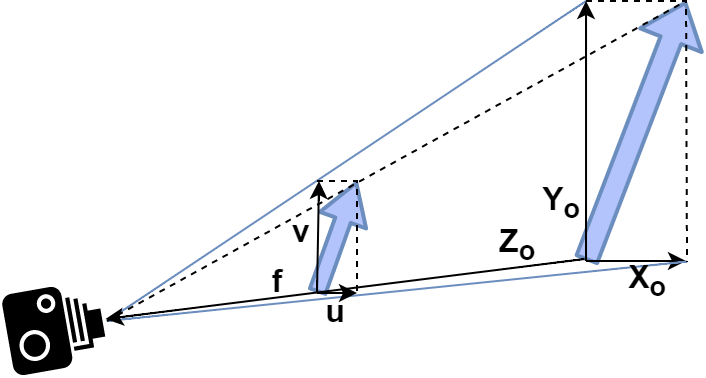
\includegraphics[width=0.5\linewidth]{"../Chap2/Figures/Camera_3D.png"}
	\caption{The pinhole camera model in 3D.} 
	\label{fig_camera3d}
\end{figure}


\subsubsection{3D Pinhole Model in Pixel Image Coordinate System}

The origin of the image coordinates is not usually set on the optical axis (i.e., at the center of the sensor, also called the principal point), but typically at its upper left (Figure~\ref{fig_imagecoord}). With $c_u$ and $c_v$ the horizontal and vertical coordinates of the principal point, the coordinates in the image frame of reference can be written as: 
\begin{equation}
  \begin{cases}
    &u = x + c_u = \frac{f\times X_C}{Z_C} + c_u\\
    &v = y + c_v = \frac{f\times Y_C}{Z_C} + c_v
  \end{cases}
\end{equation}

The relation is thus:
\begin{equation}
    Z_C \times \begin{pmatrix}u\\v\\1\end{pmatrix} = \begin{pmatrix}f & 0 &c_u \\0 & f & c_v\\0&0&1\end{pmatrix}\begin{pmatrix}X_C\\Y_C\\Z_C\end{pmatrix}
\end{equation}

\begin{figure}[hbtp]
	\centering
	\def\svgwidth{\columnwidth}
	\fontsize{10pt}{10pt}\selectfont
	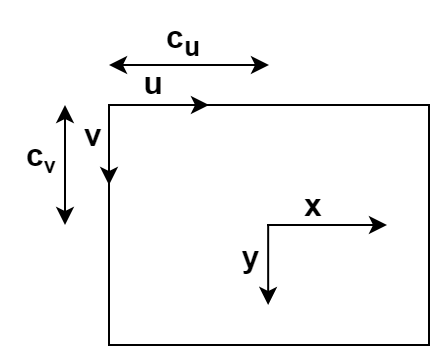
\includegraphics[width=0.3\linewidth]{"../Chap2/Figures/Image_Coord.png"}
	\caption{Image coordinates in pixel vs. sensor coordinates in meters.} 
	\label{fig_imagecoord}
\end{figure}

Moreover, instead of expressing the image coordinates and the focal length in meters, it can be convenient to express them in pixels. Let \(p_u, p_v\) be the pixel dimensions, then \(u_p = u/p_u\) and \(v_p = v/p_v\). The relation becomes:

\begin{equation}
  \begin{split}
  Z_C \times \begin{pmatrix}u_p\\v_p\\1\end{pmatrix} 
  &= \begin{pmatrix}f/p_u & 0 &c_u/p_u \\0 & f/p_v & c_v/p_v\\0&0&1\end{pmatrix}\begin{pmatrix}X_C\\Y_C\\Z_C\end{pmatrix}\\
  &= \begin{pmatrix}f_{pu} & 0 & c_{pu} \\0 & f_{pv} & c_{pv} \\ 0&0&1\end{pmatrix}\begin{pmatrix}X_C\\Y_C\\Z_C\end{pmatrix}
  \end{split}
\end{equation}


\subsubsection{3D Pinhole Model in World Coordinate System}

When several cameras are used in the same time, for instance for 3D reconstruction, it is important that they share a common frame of reference. Hence, the camera coordinate system needs to be expressed in the "world" system accordingly. Assuming that the camera is translated along a vector $T_{3\times 1}$ and rotated according to a matrix $R_{3\times 3}$, the coordinates in the camera frame of reference can be expressed in the world frame of reference as:
\begin{equation}
  \begin{pmatrix}X_C\\Y_C\\Z_C\end{pmatrix}
  = R_{3\times 3} \times \begin{pmatrix}X_W\\Y_W\\Z_W\end{pmatrix} + T_{3\times 1}
\end{equation}

\newpage
This formalism does not represent a linear system connecting the world and the camera coordinates, which can make calculations complicated. Instead, one can add one more dimension to the system and use the homogeneous coordinates, introduced by Möbius in 1927 \cite{Mobius1827}, and which constitutes one of the basis of projective geometry.
\begin{equation}\label{homogeneous}
  \begin{pmatrix}X_C\\Y_C\\Z_C\end{pmatrix}
  = \begin{pmatrix} &  & & \\ & R_{3\times 3} &  & T_{3\times 1} \\ &&&&\end{pmatrix} \begin{pmatrix}X_W\\Y_W\\Z_W\\1\end{pmatrix}
\end{equation}

Finally, the full pinhole model becomes:% (the $\textcolor{lightgray}{I_3|0}$ matrix is used to convert from the 3D to the projective space):
\begin{equation}\label{eq:pinhole}
  \boxed{
  Z_C \times \begin{pmatrix}u_p\\v_p\\1\end{pmatrix}_{\!\!3\times 1} 
  = \begin{pmatrix}f_{pu} & 0 & c_{pu}\\ 0 & f_{pv} & c_{pv} \\ 0&0&1\end{pmatrix}_{\!\!3\times 3}
    % \textcolor{lightgray}{\begin{pmatrix} &  & & 0\\ & I_{3\times 3} &  & 0 \\ &&&0&\end{pmatrix}_{\!\!3\times 4}} 
    % \begin{pmatrix} \\ & R_{3\times 3} &  & T_{3\times 1} \\  \\ 0&0&0&1\end{pmatrix}_{\!\!4\times 4} 
    \begin{pmatrix} \\ & \textbf{R}_{3\times 3} &  & \textbf{T}_{3\times 1} \\  \\\end{pmatrix}_{\!\!3\times 4} 
    \begin{pmatrix}X_W\\Y_W\\Z_W\\1\end{pmatrix}_{\!\!4\times1}
  }
\end{equation}

Or more concisely, with $\overrightarrow{q_p}$ the 2D image coordinates, $\overrightarrow{Q_w}$ the 3D world coordinates, $\textbf{K}$ the intrinsic matrix, $\textbf{H}$ the homogeneous matrix of extrinsic parameters, and $\textbf{P}$ the projection matrix:
\begin{equation}\label{eq:pinhole_short}
  \boxed{
  \begin{aligned}
  % Z_C \ \overrightarrow{q_p} &= \bm{K} \ \bm{\textcolor{lightgray}{I_3|0}} \ \bm{H} \ \overrightarrow{Q_w}\\
  Z_C \ \overrightarrow{q_p} &= \textbf{K} \ \textbf{H} \ \overrightarrow{Q_w}\\
  &= \textbf{P} \ \overrightarrow{Q_w}
  \end{aligned}
  }
\end{equation}

To sum it up, this system allows for a transformation between the coordinates of an object in meters in the world reference frame, and its coordinates in pixel on the image. It is a linear system, and thus has a closed-form solution. The intrinsic matrix $\textbf{K}$ is constant for a given camera, while the homogeneous (or extrinsic) matrix $\textbf{H}$ depends on the camera position and orientation. The projection matrix $\textbf{P}$ is the product of the intrinsic and extrinsic matrices. $Z_C$ corresponds to the distance between the camera origin and its sensor, and is considered as an arbitrary scaling factor.


\subsubsection{Skew Factor and Distortions}

Some corrections can be brought to this model. First, the pixel sides may not be perfectly perpendicular. In this case, a skew parameter $\gamma$ has to be added to the intrinsic matrix, and the relation becomes:
\begin{equation}
  Z_O \times \begin{pmatrix}u_p\\v_p\\1\end{pmatrix} = \begin{pmatrix}f_{pu} & \gamma & c_{pu} \\ 0 & f_{pv} & c_{pv} \\ 0&0&1\end{pmatrix}\begin{pmatrix}X_O\\Y_O\\Z_O\end{pmatrix}
\end{equation}
However, this is extremely rare in practice, and in the overwhelming majority of cases, $\gamma$
can safely be set to zero \cite{Zhang2000}.

\vspace*{0.5cm}
Second, the use of a lens instead of a pinhole not only introduce a finite depth of field, but also distortions. These are mostly radial, caused by the curvature of the lens, especially if it has a wide angle. Radial distortions are particularly visible when using a wide angle lens, in the form of a "barrel" effect. Straight lines are then curved near the edges of the image (Figure~\ref{fig_distortions}). Some tangential distortion can also be observed, in case the sensor is not perfectly perpendicular to the optical axis. 

These can be corrected by adding radial and tangential terms to $x$ and $y$, the image coordinates as regards to its center \cite{Weng1992}:
\begin{equation}
  \begin{cases}
  \begin{array}{rlcccc}
    x' &= x &+ &\underbrace{x(k_1 r^2 + k_2 r^4 + k_3 r^6)} &+ &\underbrace{2 p_1 x y + p_2(r^2 + 2 x^2)}\\
    &= x &+ &\Delta x_{radial} &+ &\Delta x_{tangential}\\
    \\
    y' &= y &+ &\underbrace{y(k_1 r^2 + k_2 r^4 + k_3 r^6)} &+ &\underbrace{2 p_1 x y + p_2(r^2 + 2 y^2)}\\
    &= y &+ &\Delta y_{radial} &+ &\Delta y_{tangential}
    \end{array}
  \end{cases}
\end{equation}
Where $k_1$, $k_2$, $k_3$ are the radial distortion coefficients, and $p_1$ and $p_2$ the tangential distortion ones. $r^2 = x^2 + y^2$ is the distance from the center of the sensor. This is called the DR3DT2 model, also called the Brown-Conrady distortion model \cite{Conrady1919,Brown1966}. Note that it is possible to introduce more coefficients for an even more accurate model, and that in the case of an ultra wide-angle or fisheye lens, the Kannala-Brandt model \cite{Kannala2006} is mode appropriate.

\begin{figure}[hbtp]
	\centering
	\def\svgwidth{\columnwidth}
	\fontsize{10pt}{10pt}\selectfont
	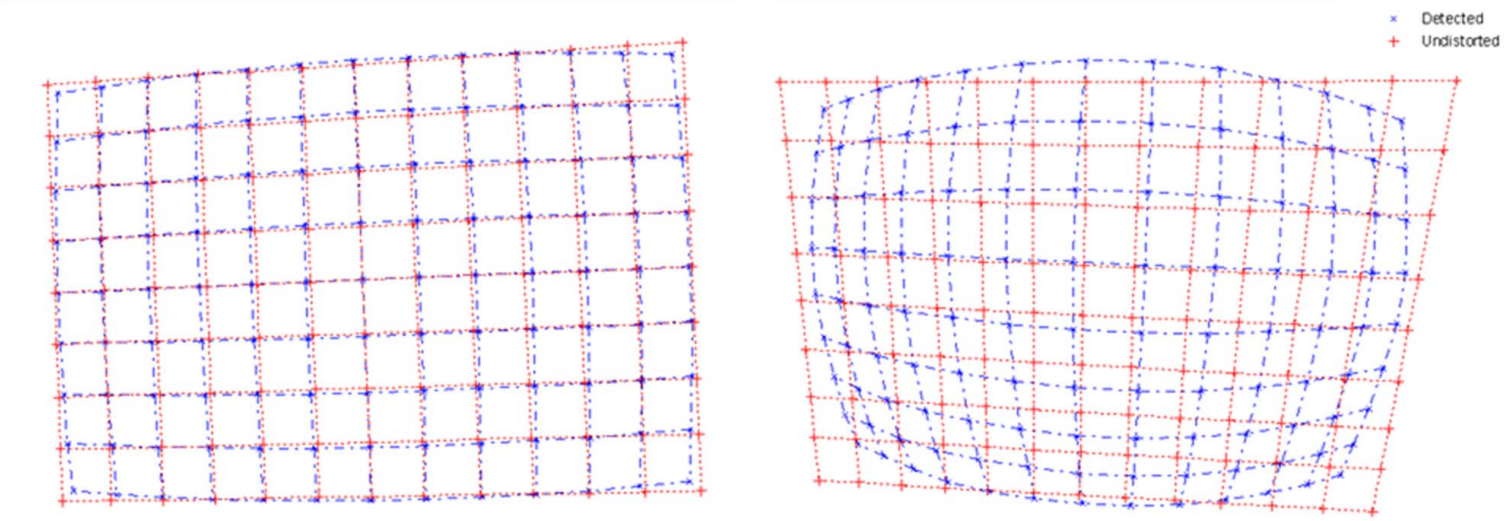
\includegraphics[width=\linewidth]{"../Chap2/Figures/Distortions.png"}
	\caption{Lens distortions are mostly radial (left image, with "barrel" effect), and sometimes tangential (right image). Image from \cite{Ricolfe2010}.} 
	\label{fig_distortions}
\end{figure}


\FloatBarrier
\subsection{Calibration}

\subsubsection{The Calibration Problem}

Camera calibration, also known as resectioning, consists of determining both intrinsic and extrinsic parameters of the camera. Extrinsic parameters are especially important to obtain for 3D reconstruction, which involves knowing the position of each camera. Intrinsic parameters can be determined at any time, however extrinsic parameters depend on the camera positions at the moment of capture, which involves that it is complicated to retrieve them afterwards -- although we proposed a method to address this issue in \autoref{ch:6}.

The intrinsic matrix is composed of 4 unknowns $f_{pu}$, $f_{pv}$, $c_{pu}$, and $c_{pv}$, while the extrinsic matrix has 3 parameters of translation, and 9 of rotation. However, the given representation of the rotation matrix is not minimal, and can be reduced to 3 parameters, for example with the Euler-Rodrigues formula \cite{Gallego2015}. Assuming no skew and no distortion, this amounts for a total of 10 unknowns. These can be determined by matching a number of points of known position in the world reference frame, to their corresponding coordinates in the image. 

\subsubsection{Direct Linear Transform (DLT) of Calibration Equations}

Considering $P_1, P_2, P_3$ the rows of the projection matrix $P$, the relation between image points and their 3D coordinates (see Equation~\ref{eq:pinhole}) can be written as \cite{Hartley2003} :
\begin{equation}\label{eq:calib_system}
  \begin{aligned}
    Z_C \times \begin{pmatrix}u_p\\v_p\\1 \end{pmatrix}_{\!\!3\times 1} 
    &= \begin{pmatrix}&&&\\&\textbf{P}&\\&&& \end{pmatrix}_{3 \times 4} 
    \begin{pmatrix} X_W \\ Y_W \\ Z_W \\ 1 \end{pmatrix}_{4\times 1}\\
    &= \begin{pmatrix}\overrightarrow{P_1} & \rule[.5ex]{3.em}{0.4pt}\\   
      \overrightarrow{P_2} &\rule[.5ex]{3.em}{0.4pt} \\ 
      \overrightarrow{P_3} &\rule[.5ex]{3.em}{0.4pt}\end{pmatrix}_{\!\!3\times 4}
      \begin{pmatrix} \vline \\ \overrightarrow{Q_W} \\ \vline \end{pmatrix}_{4\times 1}
  \end{aligned}
  \end{equation}
  Or equivalently:
  \begin{equation}
    \begin{cases}
      & Z_C \ u_p = \overrightarrow{P_1} \cdot \overrightarrow{Q_W} = \overrightarrow{Q_W^T} \cdot \overrightarrow{P_1^T}\\
      & Z_C \ v_p = \overrightarrow{P_2} \cdot \overrightarrow{Q_W} = \overrightarrow{Q_W^T} \cdot \overrightarrow{P_2^T}\\
      & Z_C \ \ \ \ = \overrightarrow{P_3} \cdot \overrightarrow{Q_W} = \overrightarrow{Q_W^T} \cdot \overrightarrow{P_3^T}\\
    \end{cases}
  \end{equation}
  We can reduce the system to two equations, and eliminate the scale factor $Z_C$:
  \begin{equation}
    \begin{cases}
      & \overrightarrow{Q_W^T} \cdot \overrightarrow{P_1^T} - u_p \ \overrightarrow{Q_W^T} \cdot \overrightarrow{P_3^T} = 0\\
      & \overrightarrow{Q_W^T} \cdot \overrightarrow{P_2^T} - v_p \ \overrightarrow{Q_W^T} \cdot \overrightarrow{P_3^T} = 0\\
    \end{cases}
  \end{equation}
  Which can be written as:
  \begin{equation}\label{eq:calib}
    \boxed{
      \begin{pmatrix}
        \overrightarrow{Q_W^T} & \overrightarrow{0^T} & - u_p \ \overrightarrow{Q_W^T}\\   
        \overrightarrow{0^T} & \overrightarrow{Q_W^T} & - v_p \ \overrightarrow{Q_W^T} \\ 
      \end{pmatrix}_{\!\!2\times 12}
      \begin{pmatrix} \overrightarrow{P_1^T} \\ \overrightarrow{P_2^T} \\ \overrightarrow{P_3^T} \end{pmatrix}_{\!\!12\times 1}
      = \begin{pmatrix} 0 \\ 0 \end{pmatrix}_{\!\!2\times 1}
    }
  \end{equation}

This operation, called Direct Linear Transform (DLT) \cite{Sutherland1974}, eliminates the $Z_C$ scaling factor, and rewrites the system in a form that allows for a resolution with linear methods. The system is composed of two equations, for 10 unknowns. Hence, it can be solved analytically with 5 corresponding image and 3D points, assuming that they are perfectly measured. This is never the case, and an approximate resolution with more points is preferred. A good rule of thumb is to measure 5 times as many points as needed, and thus to measure 25 points at least. This is classically done by using a checkerboard pattern. 

\newpage
\subsubsection{Camera Calibration from One Single Image of a Checkerboard}

The following approach is called the DLT method. Assuming that the checkerboard is used to set the origin of the world frame, the $Z_W$ coordinates are set to 0, and $X_W$ and $Y_W$ coordinates of each corner can be inferred from the dimensions of the squares. As a result, 3D coordinates of corners are known. Their 2D coordinates on the image can also be automatically detected with a subpixel accuracy, for example with the OpenCV function \href{https://docs.opencv.org/4.x/d9/d0c/group__calib3d.html#ga93efa9b0aa890de240ca32b11253dd4a}{findChessboardCorners()} \cite{Bradski2000}, which first detects edges \cite{Canny1986}, then straight lines, and then intersects the lines to obtain corner locations. Hence, 2D corners coordinates are also known. Considering M measures of matching 3D to image points, the DLT system in Equation~\ref{eq:calib} has now $2M$ equations, for 10 unknowns still:
\begin{equation}
  \begin{pmatrix}
    \overrightarrow{Q_{W1}^T} & \overrightarrow{0} & - u_{p1} \ \overrightarrow{Q_{W1}^T}\\   
    \overrightarrow{0} & \overrightarrow{Q_{W1}^T} & - v_{p1} \ \overrightarrow{Q_{W1}^T} \\ 
    \vdots & \vdots & \vdots\\
    \overrightarrow{Q_{WM}^T} & \overrightarrow{0} & - u_{pN} \ \overrightarrow{Q_{WM}^T}\\   
    \overrightarrow{0} & \overrightarrow{Q_{WM}^T} & - v_{pN} \ \overrightarrow{Q_{WM}^T} \\ 
  \end{pmatrix}_{\!\!2M\times 12}
  \begin{pmatrix} \overrightarrow{P_1^T} \\ \overrightarrow{P_2^T} \\ \overrightarrow{P_3^T} \end{pmatrix}_{\!\!12\times 1}
  = \begin{pmatrix} 0 \\ 0 \\ \vdots \\ 0 \\ 0 \end{pmatrix}_{\!\!2M\times 1}
\end{equation}

This system is now overdetermined. As it can be written in the homogeneous form \(\textbf{A} \overrightarrow{X} = \overrightarrow{0}\), a linear-eigen pseudo-solution can be found \cite{Hartley2003} by using Singular Value Decomposition (SVD) \cite{Golub1971} (See Algorithm~\ref{alg:svd}). In order to fully determine $\textbf{P}$, it first needs to be normalized, then the least-square solution needs to be found, and then it can be denormalized. 

Once the projection matrix $\textbf{P}$ has been found, it needs to be decomposed into intrinsic and extrinsic parameters, in the form:
\begin{equation} 
  \begin{aligned}
      \textbf{P} &= \textbf{K \ H} \\
                 &= \textbf{K \ (R\ \vline \ T)} \\
                 &= \begin{pmatrix}& & & &\vline & \\ && \textbf{K R}_{3\times 3} & & \vline & \textbf{KT}_{3\times 1}\\ &&&&\vline&\end{pmatrix}
  \end{aligned}
\end{equation}   
$\textbf{K}$ is an upper-triangular matrix, and $\textbf{R}$ is orthogonal by virtue of being a rotation matrix ($\textbf{R}^T$ = $\textbf{R}^{-1}$). Hence, $\textbf{K}$ and $\textbf{R}$ can be found with an RQ-decomposition (derived from QR-decomposition) from the first $3 \times 3$ block of $\textbf{P}$. This is done with Givens rotations in OpenCV, and will not be detailed here: see \cite{Bradski2000, Hartley2003} for more details. Then, finding $\overrightarrow{T}$ from the last column of $\textbf{P}$ is trivial. This decomposition can be done in OpenCV with the \href{https://docs.opencv.org/4.x/d9/d0c/group__calib3d.html#gaaae5a7899faa1ffdf268cd9088940248}{decomposeProjectionMatrix()}. However, one needs to bear in mind that this decomposition is not unique. Forcing $f_{pu}$ and $f_{pv}$ to be positive solves this issue, providing that the camera and image axes point in the same direction. 

\newpage


\begin{algorithm}[!ht]
  \caption{Linear-eigen pseudo-solution of the homogeneous system \(\textbf{A} \overrightarrow{X} = \overrightarrow{0}\)}\label{alg:svd}
  \begin{algorithmic}[1]
      \STATEx Let $\textbf{A}$ be a rectangular matrix of size $2M \times N$, composed of real or complex coefficients, and $\overrightarrow{X}$ be a vector of size $N$. The objective is to solve: 
      \begin{equation}
        \textbf{A} \overrightarrow{X} = \overrightarrow{0}
      \end{equation}
      \STATEx If $2M>N$, then the system is overdetermined, but a least-square pseudo-solution \newline
      $\overrightarrow{X^*} = argmin(\textbf{A} \overrightarrow{X})$ can be found.
      
      \STATE \textbf{A} can be factorized by Singular Value Decomposition (SVD):
      \begin{equation}
        A = \textbf{U} \ \textbf{S} \ \textbf{V}^T
      \end{equation}
      with $\textbf{U}$ an orthonormal basis of size $2M \times 2M$, \(\textbf{S}\) the rectangular diagonal matrix of \textbf{A} of size $2M \times N$, filled with its singular values \(\sigma_1, \dots, \sigma_{2M}\), and $\textbf{V}$ an orthonormal basis of size $N \times N$. $\textbf{U}$, $\textbf{V}$, and $\textbf{S}$ can be efficiently computed by the Python function \href{https://numpy.org/doc/stable/reference/generated/numpy.linalg.svd.html}{numpy.linalg.svd()}.
      
      \STATE \(\overrightarrow{X^*}\) can be expressed as a linear combination of basis vectors: 
      \begin{equation}\label{eq:xva}
        \overrightarrow{X^*} = \textbf{V} \overrightarrow{\alpha},
      \end{equation}
      with \(\overrightarrow{\alpha}\) an undetermined vector of size $N$.  
      
      \STATE \(\textbf{A}\overrightarrow{X^*}\) is close to zero where its integral \(\frac{1}{2}(\textbf{A}\overrightarrow{X^*})^2\) reaches its minimum.
      \begin{equation}
          \begin{aligned}
          (\textbf{A}\overrightarrow{X^*})^2 & = (\textbf{A} \overrightarrow{X^*})^T (\textbf{A} \overrightarrow{X^*})\\
          & = (\overrightarrow{\alpha}^T \textbf{V}^T \ \textbf{V} \textbf{S} \textbf{U}^T)(\textbf{U} \textbf{S} \textbf{V}^T \ \textbf{V}\overrightarrow{\alpha})\\
          & = \overrightarrow{\alpha}^T \textbf{S} \overrightarrow{\alpha}\\
          & = \sum_{i \in [1,N]} \alpha_i^2 \sigma_i^2
          \end{aligned}
      \end{equation}
      which is minimum when all \(\alpha\) factors are set to zero, except for the factor of the smallest singular value \(\sigma\). 

      \STATE Assuming that \(\sigma_{min} = \sigma_N\), then \((\textbf{A}\overrightarrow{X^*})^2\) is minimum when all $\alpha_i$ are null, except for $\alpha_N$.
      \begin{equation}
          (\textbf{A} \overrightarrow{X^*})_{min}^2 = \alpha_N \sigma_N
      \end{equation}
      and from equation~\ref{eq:xva}:
      \begin{equation}
          \overrightarrow{X^*} = 
          \textbf{V} \overrightarrow{\alpha} 
          = \begin{pmatrix} V_{11} & \dots & V_{1N} \\
           \vdots &  & \vdots \\
          V_{N1} & \dots & V_{NN}\end{pmatrix} \begin{pmatrix}0 \\ \vdots \\0 \\\alpha_N\end{pmatrix} 
          = \alpha_N \begin{pmatrix}V_{1N} \\ \vdots \\V_{NN}\end{pmatrix} 
      \end{equation} 
  %     \algstore{alg0}
  %   \end{algorithmic}
  % \end{algorithm}
  
  % \begin{algorithm}
  %       \begin{algorithmic}[1]
  %         \algrestore{alg0}
      \STATE Hence, $\overrightarrow{X^*}$ is solved up to a scale factor $\alpha_N$. The full system can be determined by imposing one arbitrary constraint, for example $||\overrightarrow{X^*}||=1$. 
  \end{algorithmic}
\end{algorithm}


\newpage
\subsubsection{Camera Calibration from Several Images of a Checkerboard} 

In practice, a more accurate method would use more than one single image of a checkerboard. It would also estimate distortion coefficients. A classic approach is the one proposed by \cite{Zhang2000}. It can be separated into 2 steps: first, initializing calibration parameters with a DLT method similar to the above-mentioned. Second, refining intrinsic, extrinsic, and distortion parameters by using several images of the checkerboard taken from various view points. This is treated as a non-linear optimization problem, solved by the Levenberg-Marquardt algorithm \cite{Marquardt1963,More1978} (see \hyperref[levenberg]{next section} on inverse kinematics for more details on the algorithm). The objective function that needs to be minimized is the reprojection error for all $M$ points on each $N$ checkerboard images, defined as such:
\begin{equation}\label{eq:LM_algo}
  \sum_{i \in [1,N]} \sum_{j \in [1,M]} 
  ||\ \overrightarrow{q_{ij}^{\ ^{\ ^{\ ^{\ }}}}} -
  \overrightarrow{\widehat{q_{ij}}(\textbf{K},k_1,k_2,\overrightarrow{R_i},\overrightarrow{T_i},\overrightarrow{Q_j})}\ 
  ||^2
\end{equation} 
The reprojection error is the Euclidian distance between the detected 2D point $\overrightarrow{q_{ij}}$, and $\overrightarrow{\widehat{q_{ij}}}$, the estimated projection of the 3D point $\overrightarrow{Q_j}$. Projecting 3D points on the 2D plane will be addressed in the next section on \nameref{triangulation}. In any case, $\overrightarrow{\widehat{q_{ij}}}$ is dependent on fixed intrinsic parameters (\textbf{K} matrix, distortion coefficients such as $k_1$ and $k_2$, as well as others if needed), on extrinsic parameters depending on the position of the camera when taking each checkerboard image (here, the rotation is expressed as a Rodrigues vector of size 3 \cite{Gallego2015}), and on each 3D checkerboard point. This can be done in OpenCV with the function \href{https://docs.opencv.org/4.x/d9/d0c/group__calib3d.html#ga3207604e4b1a1758aa66acb6ed5aa65d}{calibrateCamera()}, which takes matching 3D and 2D points as input, and returns extrinsic parameters for each image view, as well as intrinsic parameters and distortion coefficients.

\subsubsection{Camera Calibration with a Wand} 

In biomechanics, numerous cameras are usually needed, in order to obtain accurate 3D reconstruction in spite of occlusions. Hence, cameras are often placed around the subject. This can be problematic for the determination of a common frame of reference with a checkerboard, since it needs to be observed by all cameras simultaneously. When laying flat in the center, the checkerboard is potentially positioned at a long distance from the camera, and oriented at a challenging angle. This makes it hard for it to be detected accurately, which is consequently susceptible to deteriorate extrinsic calibration. 

On the other hand, spherical markers placed on a wand are more likely to be detected by all cameras simultaneously, regardless of their position and orientation in space. However, they only represent either a single point, or a 1D length if they are placed at both extremities of a wand. A planar object like a checkerboard, on the contrary, is sufficient to determine a 3D coordinate system. This implies that using a wand does not allow for direct 2D image point to 3D coordinate correspondences. Hence, 3D positions also need to be optimized, which involves calibrating all cameras together instead of one by one. This has a few implications: first, cameras need to be synchronized, and then, more parameters have to be optimized, which tends to make this method less stable. It should also make the optimization extremely computationally intensive. Luckily, one can take advantage of the sparsity of the Jacobian of the objective function, which allows for considerable computation savings. This method, called Sparse Bundle Adjustment (SBA), will not be described in details, but extensive explanations can be found in \cite{Lourakis2009}.

\newpage
In short, this calibration problem is solved by using a sparse variant of the Levenberg-Marquardt algorithm.  The estimated $\overrightarrow{\widehat{q_{kj}}(\overrightarrow{a_k}, \overrightarrow{b_j})}$ point is dependent on each 3D point parametrized by $\overrightarrow{b_j}$, and on each cameras image parametrized by $\overrightarrow{a_k}$. The main difference with the objective function used in the checkerboard approach, is that this one is minimized over all $M$ points of all $K$ images from all cameras, instead of for each camera independently. In order to save resources, the projection is only calculated if the point $j$ is actually visible in image $k$.

\begin{equation}
  \sum_{k \in [1,K]} \sum_{j \in [1,M]} 
  \nu_{kj} \ ||\ \overrightarrow{q_{kj}^{\ ^{\ ^{\ ^{\ }}}}} - \ 
  \overrightarrow{\widehat{q_{kj}}(\overrightarrow{a_k}, \overrightarrow{b_j})}\ 
  ||^2,  
  \textrm{ with }  
  \nu_{kj} = 
    \begin{cases}
        & 1 \textrm{ if point } j \textrm{ detected by image } k \\
        & 0 \textrm{ if unseen}
    \end{cases}
\end{equation} 


\subsubsection{In Practice}  

Both checkerboard Zhang and wand SBA methods show similar residual errors, of the order of a millimeter in a roughly $4\times 2 \times 1.5\ m^3$ capture volume \cite{Pribanic2009,Silvatti2012} (see Tables~\ref{table:tab_calib}). This is better than the classic DLT approach. Nonetheless, the wand approach does not estimate distortion coefficients as accurately as the checkerboard method. If a fisheye or a wide lens is used, the checkerboard method should be favored.

Unlike a checkerboard, wand points are visible from all angles. Moreover, the wand method has the advantage of estimating the relative position of all cameras together, and then setting the global coordinate system with another object. This represents an additional step, and it implies that cameras are synchronized, although it also means that the reference object does not need to be visible by all cameras. Conversely, with the checkerboard approach, all cameras are calibrated independently: if the checkerboard representing the global origin cannot be detected in a certain viewpoint, the corresponding camera cannot be used for 3D reconstruction. 

Nevertheless, the wand approach also optimizes over more parameters, which makes it less stable and involves a careful initialization, e.g., with an additional object of known position and dimensions, or simply by reducing the number of parameters, e.g., by fixing intrinsic parameters, which would have to be calibrated priorly. Moreover, while a checkerboard has a clearly recognizable pattern, two points of a wand are more likely to be subject to false positives errors.

In practice, a wand is much less cumbersome and much easier to transport than a checkerboard, especially for sports motion analysis where capture volumes can be large, and the checkerboard size needs to be scaled accordingly. In fact, a wand is not even necessary, and it can be replaced with the automatic detection of body segments by a 2D pose estimation model such as OpenPose \cite{Takahashi2018, Xu2021, Liu2022a}. This is, however, less accurate. The wand method is widely used by all commercial software solutions, such as Qualisys \cite{Qualisys}, as well as for free GUI such as EasyWand \cite{Theriault2014} in Matlab, or its Python version, Argus \cite{Argus,Jackson2016}. These are free, but not open-source. However, SBA is not implemented in OpenCV, and there is actually no widely supported Python version of the algorithm. Lastly, autocalibration procedures are being developed, which usually consist of automatically tracking features of interest in images, matching them across camera views, and then estimating intrinsic and extrinsic parameters in a method similar to SBA \cite{Faugeras1992,Hartley2003}. This approach is promising, but it is still in its infancy, and will not be described.

\begin{table}
	\centering
	\resizebox{\textwidth}{!}{
	\begin{tabular}{lll} 
	\toprule
	\textbf{Issue} & \textbf{Checkerboard calibration} \cite{Zhang2000} & \textbf{Wand calibration (SBA)} \cite{Lourakis2009} \\
	\specialrule{0.14 em}{0pc}{0pc}
    Accuracy & $\approx$ 1 mm  & \begin{tabular}[c]{@{}l@{}}$\approx$ 1 mm, \\unless large distorsions (e.g., fisheye)\end{tabular} \\
    	\midrule
    \begin{tabular}[c]{@{}l@{}}Transportation \& \\manipulation\end{tabular} & Large \& cumbersome & Lightweight \& foldable \\
    	\midrule
    Availability & Open-source (e.g., OpenCV) & \begin{tabular}[c]{@{}l@{}}Mostly commercial (e.g., Qualisys), or\\freeware but not open-source (e.g., Argus)\end{tabular}\\
    	\midrule
    Detection & \begin{tabular}[c]{@{}l@{}}Recognizable pattern \\but sensitive to orientation\end{tabular} & \begin{tabular}[c]{@{}l@{}}Sensitive to false positives \\but not to orientation\end{tabular}\\
    	\midrule
    GCS estimation & \begin{tabular}[c]{@{}l@{}}All cameras need to detect the reference \\object (which is sensitive to orientation)\end{tabular} & \begin{tabular}[c]{@{}l@{}}Not all cameras need to detect it, since\\camera positions known relative to each other\end{tabular}\\ 
    	\midrule    
    Optimization robustness & Robust & \begin{tabular}[c]{@{}l@{}}Need for careful initialization or \\reducing on parameters number\end{tabular}\\
    	\midrule    
    Computational cost & A few seconds & A few seconds\\
	\bottomrule
    \end{tabular}}
	\caption{Comparison of the main two approaches for accurate camera calibration: with a checkerboard \cite{Zhang2000}, or with a wand \cite{Lourakis2009}. Not that some hybrid approaches exist, e.g., those which use a checkerboard for intrinsic calibration, and a wand for extrinsic calibration. SBA: Sparse Bundle Adjustment. GCS: Global Coordinate System.}
	\label{table:tab_calib}
\end{table}

Other options, explored in \autoref{ch:6}, would be to compute intrinsic and extrinsic parameters independently. Intrinsic parameters and distortion coefficients can be calculated an any convenient moment, since they are in theory constant for a given camera. This can be done with a checkerboard, either with OpenCV raw coding, or by using a GUI like Argus \cite{Argus}. On the other hand, extrinsic parameters depend on the camera positions: they need to be computed upon every new capture setting. One way to do this consists of performing an extrinsic calibration on the spot with a wand, with fixed intrinsic parameters. Another option, if wand calibration is not possible, is to use a method analogous to Zhang's, with any 3D object of known dimensions, large enough to cover a substantial field of view for each camera. This would leverage a Perspective-n-Point approach, which consists of a Levenberg-Marquardt optimization similar to Equation~\ref{eq:LM_algo}, but with fixed intrinsic parameters \cite{Marchand2015}. This can be done with the \href{https://docs.opencv.org/4.x/d9/d0c/group__calib3d.html#ga549c2075fac14829ff4a58bc931c033d}{solvePnP} OpenCV function. 

% Matlab toolbox Bouguet J.-Y. (1999). Visual Methods for Three-Dimensional Modeling. PhD thesis, California Institute of Technology, Pasadena, CA, USA -> OpenCV = portabilité Python de Bouguet matlab ?

% Fully automatic Qualisys with passive markers if light conditions okay, EasyWand (Matlab, cite) or Argus (Python, cite) if semi-automatic tracking of color markers. GUI for all tools, otherwise raw OpenCV ?

\newpage
\subsection{Triangulation}\label{triangulation}
 
After 2D points are detected on all cameras, and considering that camera positions, orientations, and intrinsic properties are known, points can be reconstructed in the 3D space. This procedure is called triangulation, although it is a slightly abusive use of the term in case more than two cameras are used. In theory, the 3D point should lay at the intersection of all lines going from the camera centers to the 2D points (referred to as epipolar lines). In practice, the 2D points are not detected with perfect accuracy, and lines do not intersect (see Figure~\ref{fig_triangulation}). The 3D point is then approximated as the point that minimizes the distance between all epipolar lines.

\begin{figure}[hbtp]
	\centering
	\def\svgwidth{1\columnwidth}
	\fontsize{10pt}{10pt}\selectfont
	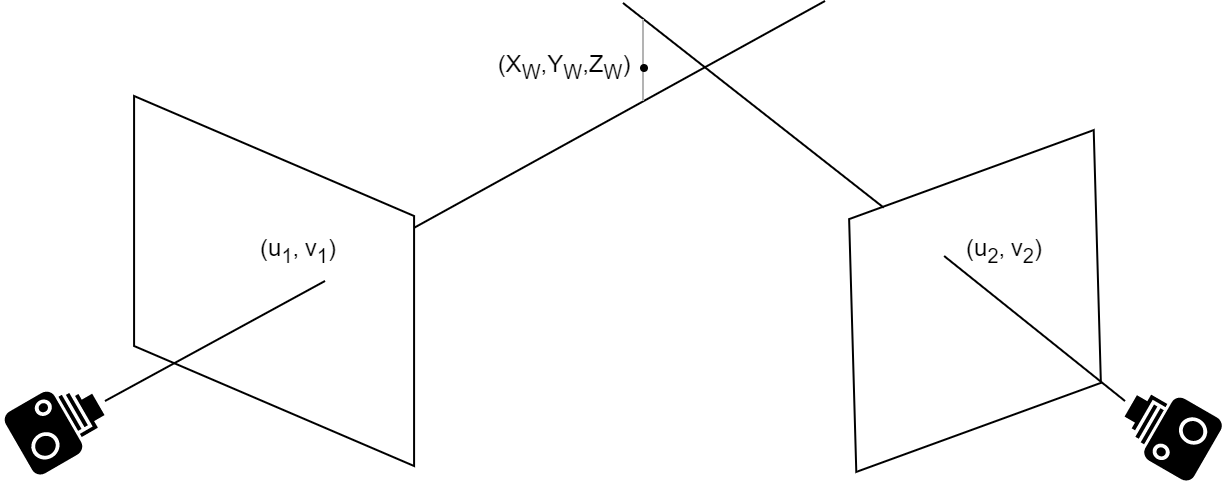
\includegraphics[width=0.7\linewidth]{"../Chap2/Figures/Triangulation.png"}
	\caption{The 3D reconstructed point can be approximated as the minimal distance between epipolar lines, which pass by each camera center and 2D detected points.}
	\label{fig_triangulation}
\end{figure}

\subsubsection{Triangulation with a Linear-Eigen Approach}  

The most straightforward, and computationally efficient method, is a DLT approach, sometimes called homogeneous or linear-eigen \cite{Hartley1997}. The procedure is slightly different from the one previously detailed for calibration. Indeed, since 3D coordinates are now the unknown variables, they are the ones factorized rather than the projection parameters. From Equation~\ref{eq:calib_system} applied to a point $\overrightarrow{Q_W}$ projected on one camera, we have:

\begin{equation}
  \begin{cases}
    & Z_C \ u_p = \overrightarrow{P_1} \cdot \overrightarrow{Q_W}\\
    & Z_C \ v_p = \overrightarrow{P_2} \cdot \overrightarrow{Q_W}\\
    & Z_C \ \ \ \ = \overrightarrow{P_3} \cdot \overrightarrow{Q_W}\\
  \end{cases}
\end{equation}
Which can be reduced as a system of two equations:
\begin{equation}\label{eq:factortrig}
  \begin{cases}
    &  (\overrightarrow{P_1} - u_p \ \overrightarrow{P_3} ) \cdot \overrightarrow{Q_W}  = 0\\
    &  (\overrightarrow{P_2} - v_p \ \overrightarrow{P_3} ) \cdot \overrightarrow{Q_W}  = 0\\
  \end{cases}
\end{equation}
Or:
\begin{equation}
  \begin{pmatrix}
      \overrightarrow{P_1} - u_p \ \overrightarrow{P_3}\\
      \overrightarrow{P_2} - v_p \ \overrightarrow{P_3}
    \end{pmatrix}_{\!\!2\times 4}
    \begin{pmatrix} X_W \\ Y_W \\ Z_W\\1 \end{pmatrix}_{\!\!4\times 1}
  = \begin{pmatrix} 0 \\0 \end{pmatrix}_{\!\!2\times 1}
\end{equation}
With C cameras, we obtain the following system of 2C equations:
\begin{equation}
\begin{pmatrix}
      \overrightarrow{P_1^1} - u_p^1 \ \overrightarrow{P_3^1}\\
      \overrightarrow{P_2^1} - v_p^1 \ \overrightarrow{P_3^1} \\ 
      \vdots \\
      \overrightarrow{P_1^C} - u_p^C \ \overrightarrow{P_3^C}\\
      \overrightarrow{P_2^C} - v_p^C \ \overrightarrow{P_3^C}
\end{pmatrix}_{\!\!2C\times 4}
\begin{pmatrix} X_W \\ Y_W \\ Z_W\\1 \end{pmatrix}_{\!\!4\times 1}
= \begin{pmatrix} 0 \\ 0 \\ \vdots \\ 0 \\ 0 \end{pmatrix}_{\!\!2C\times 1}
\end{equation}
This can be written in the form \(\textbf{A} \overrightarrow{X} = \overrightarrow{0}\), and thus a least-square solution can be found (See Algorithm~\ref{alg:svd}). Let $\textbf{V}$ be the orthonormal basis of size $4 \times 4$ obtained by SVD of $\textbf{A}$, the algorithm gives:
\begin{equation}
  \begin{pmatrix} X_W \\ Y_W \\ Z_W\\1 \end{pmatrix}_{\!\!4\times 1} 
  = \alpha_4 \begin{pmatrix}V_{14} \\V_{24} \\V_{34} \\V_{44}\end{pmatrix} 
\end{equation} 
As a consequence, the 3D coordinates of the triangulated point are:
\begin{equation}
  \boxed{
  \overrightarrow{Q_W}=\begin{pmatrix}X_W \\Y_W \\Z_W \\1\end{pmatrix} = \begin{pmatrix}V_{14}/V_{44} \\V_{24}/V_{44} \\V_{34}/V_{44} \\1\end{pmatrix}
  }
\end{equation}  

All points can be triangulated in a similar fashion, frame after frame. Since A is relatively small and the procedure relies on linear algebra, this is very fast. However, it is not robust to outliers. Other methods have been proposed, such as the Iteratively Reweighted MidPoint method (IRMP) which looks the smaller distance between all epipolar lines \cite{Yang2019}, the $L_2$ method which minimizes the sum of the squared reprojection errors \cite{Marquardt1963,More1978}, or the $L_\infty$ method which minimizes the maximum reprojection error \cite{Donne2015}, or the Q-sweep method which minimizes the median of the reprojection error, and thus is more robust to outliers \cite{Zhang2017}. Among all of these, the linear-eigen is the fastest by at least an order of magnitude, but the IRMP method may be an other good compromise in terms of speed and accuracy \cite{Chen2020b}. Some approaches also use a fast linear-eigen method, which is then refined with a (much) slower learning approach \cite{Tome2018}.

Note that these approaches do not take distortions into account, and assume either that distortions are negligible (or that the image has previously been undistorted), or that videos have been priorly undistorted based on the coefficients found during intrinsic calibration \cite{Jackson2016}. Alternatively, some action cameras such as the GoPro 5+ offer a linear mode, which undistorts videos on the fly upon capture. 

Moreover, cameras not only need to share a 3D global reference frame, but also a common time reference. Otherwise, the same frame risks relating to a different instant in the athlete's motion, in which case the 3D reconstruction would not make sense. This is classically done with a wired hardware trigger, but other approaches use a flash, a sound, or a wireless signal such as Wi-Fi, Bluetooth or GPS \cite{GoPro2022}. In \autoref{ch:6}, we proposed another approach based on cross-correlation of 2D feature speeds.

% \vspace*{0.5cm}
\subsubsection{Person Matching}  

In case of multi-person detection, an additional step needs to be undertaken prior to triangulation: the 2D detected points of each person need to be matched across all views. A common approach consists of choosing one or two keypoint (e.g., the neck and the hip), and clustering together the persons for whom epipolar lines cross at a small enough distance from each other \cite{Dong2019,Slembrouck2020,Kadkhodamohammadi2021}. This works well and efficiently, unless an epipolar line passes through several people, in the case of a crowded scene for example. In this case, it is possible to use more keypoints (or different keypoints) to solve ambiguities. Other methods use a combinatory approach, slower but more robust, which tries out all possible combinations, and minimizes the reprojection error \cite{Bridgeman2019,Chen2020c,Pagnon2021}. Other procedures use a spatio-temporal neural network, which take advantage of the information gathered in previous frames instead of working frame-by-frame \cite{Raaj2019}. Lastly, when multiple persons have been triangulated, they need to be tracked in time in order to avoid them swapping from one frame to another. This can be done by setting a threshold on 3D keypoint speed, below which a person is deemed to be correctly associated with the previous frame \cite{Bridgeman2019}.

% matching: If enough viewpoints are available, a variant of this approach uses a Random Sample Consensus (RANSAC) algorithm. It randomly takes a subset of the 2D points to be reconstructed in 3D, and 
% then tries to find the best solution for the remaining points. This is repeated several times, and the best solution is kept. This is a robust approach, but it is computationally more expensive.
% Triangulate only from best 2D estimations, called inliers, and will ignore outliers


\subsubsection{Reprojection Error}  

The reprojection error is the distance between the projection $(\widehat{u_p}, \widehat{v_p})$ of a triangulated keypoint $Q_W$ on an image, and its actual estimated 2D coordinates $(u_p, v_p)$. It can be used to jointly evaluate the accuracy of the 2D pose estimation and of the 3D reconstruction. From Equation~\ref{eq:factortrig}, we have:
\begin{equation}
    \begin{cases}
      &  \overrightarrow{P_1}\cdot \overrightarrow{Q_W} = \widehat{u_p} \ \overrightarrow{P_3} \cdot \overrightarrow{Q_W}\\
      &  \overrightarrow{P_2} \cdot \overrightarrow{Q_W} = \widehat{v_p} \ \overrightarrow{P_3} \cdot \overrightarrow{Q_W}\\
    \end{cases}
\end{equation}
Which leads to the coordinates of the reprojected point:
\begin{equation}
    \begin{cases}
      & \widehat{u_p} = \frac{\overrightarrow{P_1}\cdot \overrightarrow{Q_W}}{\overrightarrow{P_3} \cdot \overrightarrow{Q_W}}\\
      & \widehat{v_p} = \frac{\overrightarrow{P_2}\cdot \overrightarrow{Q_W}}{\overrightarrow{P_3} \cdot \overrightarrow{Q_W}}\\
    \end{cases}
\end{equation}
And then, with $\overrightarrow{\widehat{q_p}} = (\widehat{u_p}, \widehat{v_p})$ and $\overrightarrow{q_p} = (u_p, v_p)$, the mean reprojection error of this point for all C cameras can be calculated:
\begin{equation}
  \boxed{
  err = \frac{1}{C} \sum_{c \in [0,C]} ||\overrightarrow{\widehat{q_p}}-\overrightarrow{q_p}||^2 
  }
\end{equation}

Again, this formulation does not take distortions into account, so it should be taken with caution if wide lenses are used. Note that this formula is also used to calculate residual errors from calibration. Instead of reprojecting triangulated keypoints, one reprojects the 3D calibration points detected from a checkerboard or from a wand.



\newpage
\section{From 3D Pose Estimation to 3D Joint Kinematics}\label{sec:3D joint kin}

\subsection{The Kinematics Problem}

Joint kinematics is a problem which is addressed across multiple fields, including character animation, robotics, biomechanics, or even chemistry (see \hyperlink{Ann:gloss}{Disambiguation}). Each of them approaches the problem with a slightly different spirit. \cite{Robertson2013} points out that joint kinematics has proven useful across many different sports for determining "optimal movement patterns, attractor states, movement maturation, and likelihood of movement-related injury". However, reconstructed 3D keypoint coordinates alone are not enough to provide an insightful understanding of human motion. Unless some assumptions are made, one single roughly approximated keypoint per joint can at best describe planar flexion/extension angles. Even if initial 2D keypoints were accurately locating joint centers, this conceals any abduction/adduction or internal/external rotation angles. 

In order for its local coordinate system to be fully determined, a segment needs to be equipped with at least 3 non-colinear markers (see \hyperlink{Ann:gloss}{Disambiguation}). These 3 markers determine two base vectors, the third one being calculated as their cross-product. The orientation of this base coordinate system as regards to a reference one gives 3 Euler angles, commonly representing flexion/extension, abduction/adduction, and internal/external rotation of a segment. Other representations exist such as quaternions, but they still require a minimum of 3 markers per segment. Quaternions have the advantage that they are not subject to gimbal lock, however they don't correspond to any intuitive anatomical axis of rotatio;: hence, they are rarely used in the field of biomechanics. 

Now, a simplified full human body includes at least 14 segments. Consequently, at least \\$14 \times 3 = 42$ markers should be required for full-body kinematics. And yet, OpenPose and other pose estimation models only provide 25 keypoints, which are even reduced to 21 if eyes and ears are excluded. This represents half of the minimum required. For this reason, it is important to find indirect ways to obtain 3D joint angles, from seemingly incomplete information.


\subsection{The Single-Body 6DoF Approach}

The traditional method for obtaining 3D joint angles in biomechanics consists of computing positions and orientations of all body segments independently: it is called the 6DoF (6 Degrees of Freedom) free-body approach. The 6 degrees of freedom of a segment consist of 3 translations and 3 rotations, which can be determined by a 3D frame of reference, which itself assumes that there are at least 3 non-colinear markers per segment. This excludes from this paradigm most of the current pose estimation models. However, as the biomechanics community make theirs the concepts of learning-based keypoint estimation, other models with more complete labelling may arise. Therefore, for the sake of completeness, this approach is broached below.

If only 3 markers are used per segment, the problem can be solved analytically and a closed-form solution exists. The method is then called Direct Kinematics (see \hyperlink{Ann:gloss}{Disambiguation}) \cite{Lu1999}. The local reference frame of each segment can be calculated, and all inter-segmental rotations and translations can be found, using trigonometric formulas. 

In order for results to be consistent across subjects and across research studies, markers need to be carefully positioned and to follow certain standards. One of the main standards is given by the Vicon Plug-in Gait markerset for gait analysis \cite{Davis1991}, or its successor Clinical Gait Module 2 (CGM2), which has been implemented in Python as pyCGM2 \cite{Leboeuf2019b}. Strong competitors are CAST \cite{Cappozzo1995}, or its successor IOR \cite{Leardini2007}, which are implemented by the Visual3D software. For purposes more general than gait analysis, the International Society of Biomechanics (ISB) proposes a standard for both lower and upper-body analysis \cite{Wu2002, Wu2005} (see Figure~\ref{fig_isb}). Among other solutions, KineticsToolkit provides some open-source Python tools to carry out analysis according to the ISB standards \cite{Chenier2021}. 

\newpage

\begin{figure}[!ht]
	\centering
	\def\svgwidth{1\columnwidth}
	\fontsize{10pt}{10pt}\selectfont
	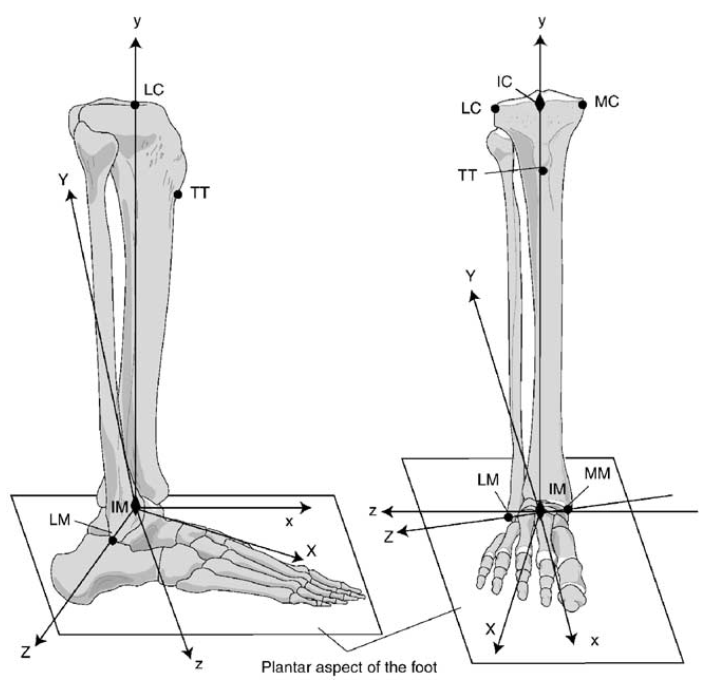
\includegraphics[width=0.7\linewidth]{"../Chap2/Figures/ISBaxis.PNG"}
	\caption{A few carefully placed markers are enough to determine the tibia/fibula coordinate system (XYZ) and the calcaneus coordinate system (xyz). Here, the ankle joint complex in the neutral position \cite{Wu2002}.}
	\label{fig_isb}
\end{figure}

If more than 3 markers are placed on the segment, the problem is overdetermined and needs to be solved numerically. The 6DoF methods is then called Single-body Kinematic Optimization (SKO), or Segmental Optimization (SO) \cite{Lu1999}. In practice, such a redundancy is advised and clusters of markers are commonly attached to body segments. It makes the analysis more robust to Soft Tissue Artifacts (STA), to measurement inaccuracies, and to potential marker loss. Let M be the number of markers of the considered segment, this segment best matches its target when all of its initial marker coordinates $\overrightarrow{X^{current}_m}$, rotated by a matrix $\textbf{R}$ and translated of a vector $\overrightarrow{T}$, are close to their measured coordinates $\overrightarrow{X^{target}_m}$. Once the local reference frame has been determined with one of the previously cited standards, minimizing the following objective function leads to a more robust approximation of the rotation and translation of the considered segment: 
\begin{equation}
  \sum_{m \in [1,M]}
  ||\ \textbf{R} \ \overrightarrow{X^{current}_m} + \overrightarrow{T} - \overrightarrow{X^{target}_m} ||^2
\end{equation} 

Each marker can be weighted with its confidence $w_m$:
\begin{equation}\label{eq:weighted_sko}
  \sum_{m \in [1,M]}
  w_m ||\ \textbf{R} \ \overrightarrow{X^{current}_m} + \overrightarrow{T} - \overrightarrow{X^{target}_m} ||^2
\end{equation} 

One way to solve it involves SVD \cite{Arun1987,Soderkvist1993} %et Veldpaus88, Challie95
, see \cite{Sorkine2017} for a step-by-step resolution. \cite{Visual3D} provides a commercial interface for SKO, and OpenSim can boil down to the same approach if 6 degrees of freedom are granted to all joints of the model.


\newpage
\subsection{The Multi-Body Inverse Kinematics Approach}\label{invkin}

\subsubsection{Principle}

Another approach is inverse kinematics, which involves considering the human body as a multi-body kinematic chain, referred to as a skeletal model. This chain is composed of segments of known length, connected with well-defined joints, each allowing a certain amount of degrees of freedom. Each segment is equipped with one or several markers, positioned at known segment coordinates. The objective of inverse kinematics is to optimize the posture of a physically consistent skeleton, scaled to each individual subject. More specifically, it aims to find the posture that minimizes the difference between model markers and measured markers. This is typically done by iteratively adjusting the joint angles of the model, until the model markers are as close as possible to the measured markers. Inverse kinematics (IK) is sometimes called Multi-body Kinematic Optimization (MKO), or Global Optimization (GO) \cite{Begon2018} (see \hyperlink{Ann:gloss}{Disambiguation}). It also represents the privileged approach to further compute joint moments, muscle activations, or inverse dynamics in general.

Inverse kinematics was first used for robotics, where joints are simple and well-defined. The typical problem consists of considering a redundant robot, which can reach one target with multiple joint configurations. This makes it an underdetermined problem. The method was then adapted for 3D animation applications, where visual coherence and fast computation matter more than accuracy. In this case, instead of just looking after the end-effector, all body segments need to be tracked. Hence, markers are usually even more numerous than the degrees of freedom, which makes it an overdetermined problem. Both cases are solved by using the same iterative optimization methods. The biomechanics community started to consider inverse kinematics as an alternative to the 6DOF one in the early 2000s, once human models became more thoroughly defined and trustworthy, and once proper individual scaling procedures were proposed \cite{Hicks2015}.

Let the Cartesian coordinates (i.e., the positions) of M markers be $\overrightarrow{X}$, and the generalized coordinates (i.e., the degrees of freedom, see \hyperlink{Ann:gloss}{Disambiguation}) of N joint angles be $\overrightarrow{q}$. The forward kinematic problem is expressed as $\overrightarrow{X}=f(\overrightarrow{q})$, and the inverse kinematics one as $\overrightarrow{q}=f^{-1}(\overrightarrow{X})$. However, $f$ is not generally invertible in practice since it is calculated as a complicated sine and cosine combination of $\overrightarrow{q}$, and therefore non-linear. Hence, optimization methods need to be leveraged. 

The objective function to minimize computes the weighted sum of the squared distances between the target measured markers $\overrightarrow{X^{target}_m}$ and the current model markers $\overrightarrow{X^{current}_m(\overrightarrow{q})}$ \cite{Lu1999}. Each degree of freedom can be subject to angle limits such as $\overrightarrow{q} \in [ \overrightarrow{q_m^{min}},\overrightarrow{q_m^{max}} ]$. Therefore, it can be expressed as:

\begin{equation}
  \sum_{m \in [1,M]}
  || \  \overrightarrow{X^{target}_m} - \overrightarrow{X^{current}_m(\overrightarrow{q})} \ ||^2
\end{equation}
\begin{equation*}
  \text{with } \overrightarrow{q} \in [ \overrightarrow{q_m^{min}},\overrightarrow{q_m^{max}} ]
\end{equation*} 
With can be written in a matrix form:
\begin{equation}\label{eq_obj_ik}
  \bigl(\overrightarrow{X^{target}} - \overrightarrow{X^{current}(\overrightarrow{q})}\bigr)^T \ 
  \bigl(\overrightarrow{X^{target}} - \overrightarrow{X^{current}(\overrightarrow{q})}\bigr)
\end{equation}
\begin{equation*}
  \text{with } \overrightarrow{q} \in [ \overrightarrow{q_m^{min}},\overrightarrow{q_m^{max}} ]
\end{equation*} 

This problem becomes increasingly hard to compute as the number of degrees of freedom increases. Consequently, iterative methods have to be employed. 3 main approaches coexist: Jacobian methods such as the Levenberg-Marquardt algorithm, Quasi-Newton methods such as the BFGS one, and Kalman filtering methods.

% is solved iteratively, using quadratic optimization \cite{Boyd2004}. Note that the term $\overrightarrow{X^{current}_m(\overrightarrow{q})}$ can be analytically computed, using forward kinematics. Since all the$\overrightarrow{q}$ parameters are optimized together, this method is robust, but slow. However, once joint angles have been optimized for the first frame, the objective function is initialized with the previous frame's joint angles, which is most likely close to the optimum, and makes optimization faster. This method is implemented in OpenSim, in the open-source Matlab toolbox CusToM \cite{Muller2019}, and in Visual3D.

\newpage
\subsubsection{Jacobian Methods and the Levenberg-Marquardt Algorithm}\label{levenberg}

In the fields of robotics and character animation, inverse kinematics is classically solved by Jacobian methods \cite{Siciliano1990,Buss2009,Aristidou2018}. They consist of linearizing marker coordinates around an initial guess on joint angles, and solving the resulting linear system. %The guess is then iteratively adjusted, until the marker coordinate error is small enough. 

Let $\overrightarrow{q^{init}}=(\theta_1^{init}, \dots \  \theta_N^{init})^T$ be the N initial joint coordinates, and \\
$\overrightarrow{X(\overrightarrow{q^{init}})} = \bigl(x_1(\overrightarrow{q^{init}}), y_1(\overrightarrow{q^{init}}), z_1(\overrightarrow{q^{init}})^T, x_2(\overrightarrow{q^{init}})^T, \dots \ z_M(\overrightarrow{q^{init}})\bigr)$ the 3M marker initial coordinates. A first order Taylor expansion of $\overrightarrow{X}$ around $\overrightarrow{q^{init}}$ yields:
\begin{equation}
    \begin{pmatrix}x_1(\overrightarrow{q^{init ^{\ }}}+\Delta\overrightarrow{q})\\ y_1(\overrightarrow{q^{init ^{\ }}}+\Delta\overrightarrow{q})\\ z_1(\overrightarrow{q^{init ^{\ }}}+\Delta\overrightarrow{q})\\ \vdots \\ z_M(\overrightarrow{q^{init ^{\ }}}+\Delta\overrightarrow{q})\end{pmatrix}_{3M \times 1}
    \approx \begin{pmatrix}x_1(\overrightarrow{q^{init}})\\ y_1(\overrightarrow{q^{init}})\\ z_1(\overrightarrow{q^{init}})\\ \vdots \\ z_M(\overrightarrow{q^{init}})\end{pmatrix}_{3M \times 1}
    + \begin{pmatrix}
        \frac{\partial{\overrightarrow{x_1(\overrightarrow{q^{init}})}}}{\partial{\overrightarrow{\theta_1}}} 
        & \cdots 
        & \frac{\partial{\overrightarrow{x_1(\overrightarrow{q^{init}})}}}{\partial{\overrightarrow{\theta_N}}} \\
        \frac{\partial{\overrightarrow{y_1(\overrightarrow{q^{init}})}}}{\partial{\overrightarrow{\theta_1}}} 
        & \cdots 
        & \frac{\partial{\overrightarrow{y_1(\overrightarrow{q^{init}})}}}{\partial{\overrightarrow{\theta_N}}} \\
        \vdots & \cdots & \vdots \\
        \frac{\partial{\overrightarrow{z_M(\overrightarrow{q^{init}})}}}{\partial{\overrightarrow{\theta_1}}} 
        & \cdots 
        & \frac{\partial{\overrightarrow{z_M(\overrightarrow{q^{init}})}}}{\partial{\overrightarrow{\theta_N}}} \\
    \end{pmatrix}_{3M\times N}
    \! \! \! \! \! \! \cdot \begin{pmatrix}\Delta\theta_1\\ \Delta\theta_2\\ \vdots \\ \Delta\theta_N\end{pmatrix}_{N \times 1}
\end{equation}
Or more formally, with \textbf{J} the Jacobian matrix of the partial derivatives of $\overrightarrow{X(\overrightarrow{q})}$ :
\begin{equation}
      \overrightarrow{X(\overrightarrow{q^{init}}+\Delta\overrightarrow{q})} 
      \approx \overrightarrow{X(\overrightarrow{q^{init}})} + \textbf{J} \ \Delta\overrightarrow{q}
\end{equation} 
The goal is to find an $\overrightarrow{X^{current}(\overrightarrow{q})} = \overrightarrow{X(\overrightarrow{q^{init}}+\Delta\overrightarrow{q})}$ which minimizes the objective function~\ref{eq_obj_ik}. The function can then be expressed as:
\begin{equation}
  \Bigl(\overrightarrow{X^{target}} - \overrightarrow{X(\overrightarrow{q^{init}})} - \textbf{J} \ \Delta\overrightarrow{q} \Bigr)^T \ 
  \Bigl(\overrightarrow{X^{target}} - \overrightarrow{X(\overrightarrow{q^{init}})} - \textbf{J} \ \Delta\overrightarrow{q} \Bigr)
\end{equation}
Or more simply, with $\Delta\overrightarrow{X} = \overrightarrow{X^{target}} - \overrightarrow{X(\overrightarrow{q^{init}})}$, as:
\begin{equation}
  (\Delta\overrightarrow{X} - \textbf{J} \ \Delta\overrightarrow{q} )^T \ 
  (\Delta\overrightarrow{X} - \textbf{J} \ \Delta\overrightarrow{q} )
\end{equation}
It is minimum when its gradient is annulled, i.e., when:
\begin{equation}
  \begin{aligned}
   \overrightarrow{0} &\approx 
   \frac{\partial}{\Delta \overrightarrow{q}}
   \Bigl( ( \Delta\overrightarrow{X} - \textbf{J} \ \Delta\overrightarrow{q})^T \ 
  (\Delta\overrightarrow{X} - \textbf{J} \ \Delta\overrightarrow{q} ) \Bigr)  \\
  & = - \textbf{J}^T \ 
  (\Delta\overrightarrow{X} - \textbf{J} \ \Delta\overrightarrow{q} ) 
  + (\Delta\overrightarrow{X} - \textbf{J} \ \Delta\overrightarrow{q} )^T 
  (-\textbf{J})\\
  & = -2 \textbf{J}^T \ 
  (\Delta\overrightarrow{X} - \textbf{J} \ \Delta\overrightarrow{q} )
  \end{aligned}
\end{equation}
Which is when:
\begin{equation}
  \Delta\overrightarrow{X} \approx \textbf{J} \ \Delta\overrightarrow{q}
\end{equation}
Each marker can be weighted more or less according to its level of trust. Typically, markers placed on large muscle or fat tissues (such as thighs)are subject to strong STA, and will therefore be weighted less than those placed on bony landmarks (such as ankle malleoli). Hence, marker coordinates will be multiplied by the diagonal matrix of weights \textbf{W} \cite{Meredith2005}:
\begin{equation}
  \boxed{
  \textbf{W} \ \Delta\overrightarrow{X} \approx \textbf{J} \ \Delta\overrightarrow{q}
  }
\end{equation}

\vspace*{0.5cm}
Now, the change in joint angles needed to reach the target from the current position can be found by calculating $\Delta \overrightarrow{q} \approx \textbf{J}^{-1} \textbf{W} \ \Delta\overrightarrow{X}$. However, \textbf{J} is typically not invertible. Several optimization approaches can be used to approximate this inversion. For all of them, the idea is to evaluate the marker coordinate error $\Delta\overrightarrow{X}$, then approximately calculate the corresponding joint angle error $\Delta \overrightarrow{q}$ and correct it, then reevaluate the marker coordinate error, etc. until it stays below a satisfying threshold.

\begin{enumerate}[itemsep=0em, topsep=0em, leftmargin=*]
    \item \textbf{Using the Jacobian transpose $\textbf{J}^T$} to roughly approximate the trend, with a small relaxation factor $\alpha$ (which can be optimally calculated \cite{Buss2009}):
    \begin{equation}
      \Delta \overrightarrow{q} \approx \alpha \textbf{J}^T \ \textbf{W} \ \Delta\overrightarrow{X}
    \end{equation} 
    This is analogous to the \emph{gradient descent method} \cite{Nocedal1999}. $\textbf{J}^T$ is quick and easy to compute, but the algorithm converges slowly, and pose results are sometimes unsatisfying.
    
    \item \textbf{Using $\textbf{J}^+$, the Moore-Penrose pseudo-inverse of J}. Left-multiplying by $\textbf{J}^T$ gives:
    \begin{equation}
        \textbf{J}^T \ \textbf{W} \ \Delta\overrightarrow{X} \approx \textbf{J}^T \textbf{J} \ \Delta\overrightarrow{q}\\
    \end{equation}
    $\textbf{J}^T \textbf{J}$ has full rank, so it is invertible:
    \begin{equation}\label{eq:pseudoinv}
      \begin{aligned}
        \Delta \overrightarrow{q} &\approx \ (\textbf{J}^T \textbf{J})^{-1} \textbf{J}^T \ \textbf{W} \ \Delta\overrightarrow{X} \text{, i.e.,} \\
        \Delta \overrightarrow{q} &\approx \textbf{J}^+ \ \textbf{W} \ \Delta\overrightarrow{X} 
      \end{aligned}
    \end{equation} 
    This is analogous to the \emph{Gauss-Newton method} \cite{Nocedal1999}. This method converges faster, but is sensitive to bad initial estimates and unstable near singularities of $\textbf{J}^+$, i.e., when $\Delta \overrightarrow{q}$ becoming unreasonably for a small $\Delta \overrightarrow{X}$ shift. Moreover, the pseudo-inverse can be expensive to compute. One way to mitigate this drawback consists of calculating it with an SVD. The Jacobian can be decomposed as $\textbf{J} = \textbf{U} \ \textbf{S} \ \textbf{V}^T$ (see Algorithm~\ref{alg:svd}). Then:
    \begin{equation}
          \begin{aligned}
          \textbf{J}^+
          & = (\textbf{J}^T \textbf{J})^{-1} \textbf{J}^T \\
          & = (\textbf{V} \ \textbf{S}^T \cancel{\textbf{U}^T} \ \ \
          \cancel{\textbf{U}} \ \textbf{S} \ \textbf{V}^T)^{-1} \ \  
          \textbf{V} \ \textbf{S}^T \textbf{U}^T \ \ \\
          & = (\textbf{V} \ \textbf{S}^T\textbf{S}\ \textbf{V}^T)^{-1} \ \  
          \textbf{V} \ \textbf{S}^T \textbf{U}^T \ \ \\
          & = \textbf{V} (\textbf{S}^T\textbf{S})^{-1} \cancel{\mathbf{V^T}} \ \  
          \cancel{\textbf{V}} \ \textbf{S}^T \textbf{U}^T \ \ \text{, since }\textbf{V}^{-1}=\textbf{V}^T\\
          & = \textbf{V} \ \textbf{S}^{+} \textbf{U}^T \ \ \\
        \end{aligned}
      \end{equation}
      And 
      \begin{equation}
        \Delta \overrightarrow{q} \approx \textbf{V} \ \textbf{S}^{+} \textbf{U}^T \ \textbf{W} \ \Delta\overrightarrow{X} 
      \end{equation}

    \item \textbf{Using the Levenberg-Marquardt (LM) algorithm} \cite{More1978}, also called the Damped Least-Square (DLS) method, and slightly adjusting Equation~\ref{eq:pseudoinv}:
    \begin{equation}
        \Delta \overrightarrow{q} 
        \approx \ (\textbf{J}^T \textbf{J} + \lambda^2 \textbf{I})^{-1} \textbf{J}^T \ \textbf{W} \ \Delta\overrightarrow{X}
    \end{equation} 
    This is an intermediary method, which is stable near singularities and robust to bad initial estimates like the gradient algorithm when the damping factor $\lambda$ is large, and converges fast like the Gauss-Newton algorithm when $\lambda$ is small. $\lambda$ has to be chosen carefully, but can also be adjusted after each iteration. Again, the matrix is costly to invert, but it is possible to use SVD to decrease the computational complexity. One can demonstrate that:
     \begin{equation}
        \begin{array}{rlccccc} 
            (\textbf{J}^T \textbf{J} + \lambda^2 \textbf{I})^{-1} \textbf{J}^T 
            &\approx& \textbf{V} \ & \underbrace{\textbf{S}^{+} (\textbf{S} \textbf{S}^T+\lambda^2 \textbf{I})} \  & \textbf{U}^T \ \ \\
            & = & \textbf{V} & \ \textbf{E}^{+} & \  \textbf{U}^T
        \end{array}
     \end{equation}
    And 
      \begin{equation}
        \Delta \overrightarrow{q} \approx  \textbf{V} \ \textbf{E}^{+} \textbf{U}^T \ \ \textbf{W} \ \Delta\overrightarrow{X}
      \end{equation}
\end{enumerate}

In plain words, the gradient descent method iteratively searches the direction of steepest gradient, until the objective function reaches a minimum where the gradient is null; while the Gauss-Newton method linearizes the problem, takes advantage of the sum-of-squares formulation of the objective function, and directly finds where the gradient vanishes; and the Levenberg-Marquardt method is a compromise between the two.

Jacobian-based methods use the result of the previous frame as an initial guess, which is arguably close to the desired solution. Hence, they are generally fast and can be used in real-time in 3D animation software applications. However, they can produce oscillation motion with discontinuities and jerky movements, especially near singularities, and tend to be less precise than Quasi-Newton methods \cite{Aristidou2018}. Moreover, joint limits are not straightforward to take into account, and such constraints tend to slow the convergence rate and to lead to poorer accuracy \cite{Aristidou2018}. The Levenberg-Marquardt method is implemented in the open-source softwares Pyomeca \cite{Martinez2020} with the Biorbd library \cite{Michaud2021}, \cite{Pinocchio,Carpentier2019}, CusToM \cite{Muller2019}, as well as in Visual3D. 


\subsubsection{Quasi-Newton Methods and the BFGS Algorithm}

In the field of biomechanics, inverse kinematics is usually dealt with more general Quasi-Newton methods. These methods don't linearize the objective function, and solve it as a more general non-linear minimization problem, which is not restricted to sum-of-squares objective functions. 
% Note that in this sense, the Gauss-Newton method is a Quasi-Newton method applied to a specific class of problems. 
Let us call $h(\overrightarrow{q})$ be the objective function~\ref{eq_obj_ik} to minimize. A second order Taylor expansion of $h$ around $\overrightarrow{q}$ is:
\begin{equation}
      h(\overrightarrow{q}+\Delta\overrightarrow{q}) 
      \approx h(\overrightarrow{q}) \ 
      + \overrightarrow{\nabla h(\overrightarrow{q})}^T  \ \Delta\overrightarrow{q} \ 
      + \frac{1}{2}  \ \Delta\overrightarrow{q}^T \ \bm{\nabla^2 h(\overrightarrow{q})}  \ \Delta\overrightarrow{q}
\end{equation} 
Where $\overrightarrow{\nabla h(\overrightarrow{q})}$ is the gradient vector of h with respect to $\overrightarrow{q}$, and $\bm{\nabla^2 h(\overrightarrow{q})}$ its Hessian matrix. This functional is minimum when its gradient (with respect to $\Delta\overrightarrow{q}$) is null.
\begin{equation}
    \begin{aligned}
      \overrightarrow{0} &\approx 
      \frac{\partial}{\Delta \overrightarrow{q}}
      \Bigl( h(\overrightarrow{q}+\Delta\overrightarrow{q}) \Bigr) \\
      &\approx
      \nabla h(\overrightarrow{q})^T  \  
      + \Delta\overrightarrow{q}^T \ \bm{\nabla^2 h(\overrightarrow{q})}
    \end{aligned}
\end{equation} 
So:
\begin{equation}
    \Delta\overrightarrow{q}
    = - \Bigl( \bm{\nabla^2 h(\overrightarrow{q})}\Bigr)^{-1} \ \nabla h(\overrightarrow{q})
\end{equation}      

Hence, this method is similar to the Gauss-Newton one, in the sense that it directly searches for where the gradient vanishes. However, it does not take advantage of the sum-of-squares formulation of the problem, and requires inverting its Hessian matrix of second derivatives, which is very computationally expensive. In Quasi-Newton methods, the Hessian is approximated by a matrix \textbf{B}, which is updated after each iteration. One of the most common approximation method is the BFGS one, found independently by 4 different researchers in the same year, 1970. Its precise formulation can be found in \cite{Nocedal1999}.

More specifically, in the field of inverse kinematics, the L-BFGS-B variant is often used. This is a limited-memory of the BFGS method, which uses a sparse approximation of the Hessian instead of a dense one, further adapted for handling joint limits by gradient projection \cite{Byrd1995,Zhao1994}. Since the Jacobian is not inverted, these methods return the smoothest and most accurate results, and stay free from any singularity issues like with the Levenberg-Marquardt method. However, they are still more computationally costly than Jacobian methods, and are not as straightforward to implement \cite{Aristidou2018}. They are used in the open-source software applications OpenSim, and in Visual3D. Pyomeca \cite{Martinez2020} relies on the OpenSim Python API to provide such a method, via its library Pyosim. CusToM uses a Sequential Quadratic Programming method, which is a generalization of constrained Newton ones. It is slower, and arguably not necessary for simple bound constraints.


\newpage
\subsubsection{Kalman Filtering Methods}

Another lesser-known class of inverse kinematic methods is the Kalman filter, which does not take its roots from the fields of robotics, nor computer animation, nor biomechanics, but from automation. In fact, it was precisely designed to mitigate the effect of noisy measurement data on the estimation of variables of interest \cite{Kalman1960}. Kalman filters don't involve the definition of any objective function, however they take advantage of prior knowledge of both the evolution of kinematic variables along time (namely, the process model), and of the kinematic chain (namely, the measurement model). The process model concerns the change of state variables from one frame to another, as well as the magnitude of imprecision on their predicted evolution. State variables are primarily joint angles, but they can also include their derivatives up to an arbitrary number (although \cite{DeGroote2008} showed that little improvement was brought when going above the 2nd degree), marker coordinates, IMU inputs, etc. The measurement model defines the relationship between marker positions and state variables, as well as the magnitude of errors (due to STA for example). 

In short, an inverse kinematics Kalman filter will proceed in two steps. It will first predict the angular joint parameters of the next frame thanks to the process model. Then, it will update this prediction, by deducing the corresponding marker positions thanks to the process model, and comparing these to the actual measured marker coordinates. This difference will be weighted by the Kalman gain, computed at each frame, and added to the initial joint parameter estimate. 

\vspace*{0.5cm}
\noindent\textbf{Prediction phase:}

Let $\overrightarrow{q} = (\theta_1, \dot{\theta_1}, \ddot{\theta_1}, \theta_2, \cdots, \ddot{\theta_N})^T_{1 \times 3N}$ be the joint angle coordinates, velocities, and accelerations, called the state vector. The \emph{process model} is expressed as: 
\begin{flalign}
    &&\fbox{$\overrightarrow{q(t+\Delta t)} 
    = f\bigl(\overrightarrow{q(t)}\bigr) + \overrightarrow{\eta(t)}$},
    && \text{with } \overrightarrow{\eta(t)} \sim \mathcal{N}(0,\,Q_t)&&
\end{flalign}
$\overrightarrow{\eta(t)}$ is the process noise, assumed to be a zero-mean Gaussian distribution with covariance $\textbf{Q}_t$. Considering that the mean process noise is null, an estimate for $\overrightarrow{q(t+\Delta t)}$ is:
\begin{equation}
    \overrightarrow{\hat{q}(t+\Delta t)} 
    = f\bigl(\overrightarrow{q(t)}\bigr)
\end{equation}
As f is a combination of multiple sine and cosine functions, it is not linear. Let n refer to any of the N joint angles, a second order Taylor expansion can help linearize the problem:
\begin{equation}
    \begin{pmatrix}\hat{\theta}_n(t+\Delta T)\\ \hat{\dot{\theta}}_n(t+\Delta T)\\ \hat{\ddot{\theta}}_n(t+\Delta T)\end{pmatrix} 
    \approx \begin{pmatrix}1 & \Delta t & \Delta t^2/2 \\0 & 1 & \Delta t\\0&0&1\end{pmatrix}
    \begin{pmatrix}\theta_n(t)\\ \dot{\theta}_n(t)\\ \ddot{\theta}_n(t)\end{pmatrix} 
\end{equation}
Or more succinctly, predicted joint angular parameters are: 
\begin{equation}
    \overrightarrow{\hat{q}(t+\Delta t)} 
    = \textbf{F}\ \overrightarrow{q(t)}
\end{equation}
The covariance of prediction $\hat{\textbf{P}}_{t+\Delta t}$ is also calculated at this stage. As it is lengthy to expose and slightly convoluted, we won't detail it here (see \cite{Bonnet2017a} for further details on its determination). 


\vspace*{0.5cm}
\noindent\textbf{Update phase:}

Let $\overrightarrow{X} = (x_1, y_1, z_1, x_2, \cdots, z_M)^T_{1 \times 3M}$ be the measured marker coordinates, called the output vector. The \emph{measurement model} is expressed as: 
\begin{flalign}
    &&\fbox{$\overrightarrow{X(\overrightarrow{q(t)})}
    = h\bigl(\overrightarrow{q(t)}\bigr) + \overrightarrow{\nu(t)}$},
    && \text{with } \overrightarrow{\nu(t)} \sim \mathcal{N}(0,\,R_t)&&
\end{flalign}
$\overrightarrow{\nu(t)}$ is the zero-mean measurement noise of covariance $\textbf{R}_t$. The update phase starts with computing the difference between measured marker positions $\overrightarrow{X^{target}}$, and those deducted from the measurement model:
\begin{equation}
    \Delta \overrightarrow{X(t+\Delta t)} 
    = \overrightarrow{X^{target}(t+dt)}
    - h\bigl(\overrightarrow{\hat{q}(t+\Delta t)}\bigr)
\end{equation}
The covariance of error $\textbf{S}_{t+\Delta t}$ is more complicated to compute: as $h$ is non-linear, it has to be approximated with a first order Taylor expansion. Both prediction and error covariances $\hat{\textbf{P}}_{t+\Delta t}$ and $\textbf{S}_{t+\Delta t}$ are involved in the computation of the Kalman gain $\textbf{K}_{t+\Delta t}$.

Finally, the updated joint parameter estimates are:
\begin{equation}
\boxed{
    \Delta \overrightarrow{q(t+\Delta t)} 
    = \overrightarrow{\hat{q}(t+\Delta t)} 
    + \textbf{K}_{t+\Delta t} \ \Delta \overrightarrow{X(t+\Delta t)} }
\end{equation}
A low Kalman gain means that the initial estimate can be trusted, and a higher gain places more weight on marker measurements.

\vspace*{0.5cm}
The Kalman filter (KF) deals with linear problems, and joint kinematics is highly non-linear. Other methods have been derived to broadens its usage to non-linear cases, such as the Extended Kalman Filter (EKF), which was first introduced for joint kinematic estimation by \cite{Cerveri2003}. The Local Marker Estimation filter (LME) compensates for Soft Tissue Artifacts (STAs) \cite{Cerveri2005,Bonnet2017a}. The Kalman Smoother (KS) filters both ways, from first to current frame, and from last to current frame \cite{Rauch1965}. It can also be extended in the non-linear case, and is then called the Extended Kalman Smoother (EKS). It results in smoother and more accurate estimation of joint kinematic variables \cite{DeGroote2008}. However, this is at the cost making the analysis off-line, while Kalman filters have the potential of being used in real-time. 

Kalman-based methods take advantage of prior knowledge on the expected evolution of joint variables in time, on the kinematic chain, and they also take noise into account. If fact, it has been demonstrated that the Levenberg-Marquardt algorithm is a specific case of the extended Kalman filter, which results under simplifying assumptions \cite{Bell1994,Horvath2016}. Consequently, Kalman-based methods have been shown to be more accurate in general than Jacobian-based and Quasi-Newton methods \cite{Cerveri2005,DeGroote2008, Bonnet2017a}, although some studies found similar results \cite{Fohanno2014}. In any case, they are especially accurate for the estimation of velocities and accelerations \cite{Fohanno2014}, since they are directly estimated by the filter, without further differentiation which would introduce additional errors. This is especially interesting for the study of forces, which can be estimated based on accelerations. They are more robust to decreased number of markers \cite{Fohanno2010}. With the exception of KS, they can also work in real time \cite{Fohanno2014}. 

However, since joint kinematic variables are estimated from the previous frame, a Kalman filter requires an initial guess on joint angular coordinates, velocities, accelerations, and covariances. Initial velocities and accelerations are usually assumed to be zero, but this is not always the case, especially when capturing sports movements. Moreover, the setup of the covariance factors is still an open issue. According to \cite{Cerveri2005}, those associated to the measurement (marker coordinates) need to be at least 2 orders of magnitude lesser than the ones of the process (joint parameters). As a reference, Biorbd \cite{Michaud2021}, a library used by Pyomeca \cite{Martinez2020}, uses a process factor $\sigma^2_p=10^{-10}$ and a measurement factor $\sigma^2_m=10^{-5}$, while a fork of OpenSim \cite{DeGroote2008} takes default standard deviations of $\sigma_p=15$ and $\sigma_m=0.03$.

Similarly to Jacobian methods, and unlike with Quasi-Newton ones, most types of constraints are not straightforward to implement. Constraints on the number of degrees of freedom are naturally introduced with the definition of the measurement model \cite{Halvorsen2008}. Hard joint limit constraints can be implemented by saturating the Kalman gain if the first joint estimate is not within limits, and then by recomputing the estimation \cite{Bonnet2017b}. Soft closed-loop constraints can be handled by introducing penalties near joint limits \cite{Fohanno2014}.

An Extended Kalman Filter is implemented in Pyomeca with its Biorbd library \cite{Michaud2021}, and a Kalman Smoother has been proposed in a fork of OpenSim \cite{DeGroote2008}.

% Hidden markov, but continuous instead of discrete space 


\subsubsection{Other Inverse Kinematic Methods}

Other methods have been proposed, which can be divided into the heuristic and the learned ones. Heuristic methods consist of trying to reach targets by considering only one joint at a time, instead of minimizing an objective function on marker coordinates or filtering joint angle evolution. 

Cyclic Coordinate Descent (CCD) consists of minimizing the distance between the end-effector and the target, by freeing one degree of freedom after another \cite{Wang1991}. It is very fast and simple to implement, including with joint limits \cite{Welman1993}. However, it results in abrupt movements, and the last joints can be unnaturally twisted. It is not really applicable beyond a few joints, nor if numerous markers are used, instead of just an end-effector. CCD is not usually considered suitable for biomechanical analysis, and currently remains primarily limited to the field of computer animation \cite{Kulpa2005}. 

Forward And Backward Reaching IK (FABRIK) starts by moving the end-effector directly on the target, and adjusts the positions of other joints so that they respect segment dimensions, and remain close to their previous position. The same maneuver is then reproduced, starting from the first joint, and repeated until success \cite{Aristidou2011}. It is fast, robust, supports joint limits, and can be used with multiple end-effectors. However, each joint is treated independently and the algorithm does not have a global overview of the system, which can lead to a deadlock situation in some cases. This has been partly solved by introducing random pertudbations \cite{Aristidou2016}. Overall, heuristic methods are very fast, but can be bear unacceptable limitations, especially with complex models and when accuracy is the main concern.

Learned approaches are data-driven rather than knowledge-driven. Instead of striving to search for the posture which matches marker positions and constraints the best, they leverage neural networks, using the numerous available databases gathered along time. Among them, deep-learning methods have lately been integrated for human pose reconstruction. Many approaches exist, most of them specifically estimating angle outputs from a target coordinate input \cite{Mordatch2015,Du2015}. However, these methods usually require prior training, are computationally intensive to use, and can only work properly if they are used on data which are sufficiently close to the training dataset. They are still in their infancy and to our knowledge, have not been tested for biomechanical applications yet.


\subsection{6DoF vs. Inverse Kinematics}

Ultimately, the main difference between the free-body 6DoF approach and the multibody inverse kinematic one boils down to the idea that in order to conduct a 6DoF analysis, one needs to trust markers, while for IK one needs to trust the model (see Table~\ref{table:tab_kin}). \cite{Moniz2014} found that for the elderly, RMSD between both approaches remained under 5° for all lower-body joints, except for hip and ankle internal/external rotation, respectively 12° and 7°. For children with cerebral palsy, results were similar, and as long as segments bore the same anatomical frames of reference, the RMSD stayed under 4°, aside from hip and ankle internal/external rotation which still remained under 6°. For the knee analysis of American football players, \cite{Robinson2013} found up to 11° RMSD for the abduction/adduction angle, and 7° for internal/external rotation. However, both approaches classified the same athletes as being at risk injury. Hence, in a lot of cases, results are comparable. Note that due to the dearth of available gold-standard data, it is difficult to compare the accuracy of both approaches aside from computer simulated experiments.

If the 6DoF approach is used, one single trained operator needs to position markers, very accurately and consistently. At least 3 markers need to be tracked on each segment. The effect of Soft Tissue Artifacts is noticeable, even when their local frame coordinates are optimized by using more than 3 markers per segment. However, this approach is not computationally intensive and can be run in real-time. It does not require any joint center calculation, individual scaling procedure, nor any geometric assumption. In fact, it is not based on a model, which is an advantage when studying a population that is pathological or outside the norms. The 6DoF approach can also render joint dislocations, which is desirable if joint laxity is a parameter that is specifically of interest. On the other hand, this comes with the drawback that segments can interpenetrate each other, or even change length.

If the inverse kinematic method is used, a model first needs to be designed. Although we just glanced over this aspect, it is not trivial. It involves correctly modeling joints, with the appropriate degrees of freedom or coupling relationships, and requires scaling the model to each individual person. This is usually done by adjusting segments dimensions according to distances between joints, and thus joint center coordinates need to be estimated. Joint centers are often defined as the midpoint between anatomical markers for ankles, knees, elbows, and wrists, but these methods are not always accurate, and sometimes not workable at all, for instance in the cases of the hip or the shoulder joint. In these cases, functional methods such as SCoRE for ball joints \cite{Ehrig2006} or SARA for hinge joints \cite{Ehrig2007} are leveraged. These methods require the subject to perform a set of predefined movements prior to the actual capture, which is time-consuming. Moreover, the mere concept of joint centers is also not always pertinent, especially for the shoulder girdle or for the knee, which allow for both rotations and translation motions \cite{Seth2010}. 

The IK approach assumes that all human beings have similar joint mechanics, based on \textit{a priori} constraints inferred from non-exhaustilve observations. Hence, it can be difficult to implement for pathological populations nor on unusual body structures: for instance, joint laxity cannot be qualified. Hence, the model must be carefully designed before granting trust to results \cite{Hicks2015}. 

On the other hand, inverse kinematics has been reported to be more accurate than 6DoF, as it is less sensitive to STAs as it addresses them globally, and as it does not suffer from interpenetration or length changes. It reduces the number of degrees of freedom to solve, and thus of markers needed \cite{Slater2018}. Note that inverse kinematics is equivalent to 6DoF if all joint degrees of freedom are released. Using a model can also be the starting point for further analysis, such as muscle activation for example \cite{Robinson2013,Kainz2016}.

This approach is generally computationally intensive, and can only be run in real-time if the model is simple. This issue is not as critical nowadays as it used to, as computing capabilities are growing exponentially with time, according to Moore's law \cite{Moore1965}, and as algorithms have been improved to decrease their computational complexity. 

\cite{Aristidou2018} states that the 6DoF approach should be favored if the model is simple, with little risk of STA, or if looking at pathological individuals. A standard model may not fit well to these persons, and some clinically relevant movements such as joint dislocations could be missed. These approaches are also much faster to compute, and can be conducted in real-time. On the other hand, the IK approach should be favored with a more general population, especially if their body fat or muscles are considerable enough to cause large STA.

The most exact IK methods are the Kalman methods, and they are also fast. However, they are difficult to initialize, and can diverge if the initial estimates are not accurate enough. In particular, there is no consensus on the values of covariances. Jacobian methods such as Levenberg-Marquardt are also fast, generally robust on most joint configurations, but they are also subject to divergence around singularities. Consequently, in the field of biomechanics, the most used methods are the Quasi-Newton ones, such as L-BFGS-B which is implemented in OpenSim. They are slower, but also more accurate, more robust to bad initial estimates, and they additionally better handle joint limits. 


\begin{table}[!htbp]
  \centering
  \resizebox{1\textwidth}{!}{
  \begin{tabular}[t]{llll}
  \toprule
  &\multicolumn{3}{c}{\textbf{Single-body 6DoF}} \\
  \midrule
                    & \multicolumn{3}{c}{\textbf{\emph{Involves trusting marker coordinates}}} \\
                    & \multicolumn{3}{c}{In most cases, results comparable to IK} \\
  Pros and Cons     & \multicolumn{3}{l}{\hspace{10em}+ Simplest to implement} \\
                    & \multicolumn{3}{l}{\hspace{10em}+ Fastest to compute} \\
                    & \multicolumn{3}{l}{\hspace{10em}+ More appropriate with population outside the norm} \\
                    & \multicolumn{3}{l}{\hspace{10em}+ No need for any model} \\
                    & \multicolumn{3}{l}{\hspace{10em}- Not always accurate} \\
                    & \multicolumn{3}{l}{\hspace{10em}- 3 markers per segment at least} \\
                    & \multicolumn{3}{l}{\hspace{10em}- Sensitive to STAs} \\
                    & \multicolumn{3}{l}{\hspace{10em}- Segments can change dimensions and interpenetrate} \\
    Solutions       & \multicolumn{3}{l}{\hspace{10em}\emph{OpenSim \cite{Delp2007}}}\\ 
                    & \multicolumn{3}{l}{\hspace{10em}\emph{KineticsToolkit \cite{Chenier2021}}}\\ 
                    & \multicolumn{3}{l}{\hspace{10em}\emph{\cite{Visual3D}$^1$}} \\
  \specialrule{0.14 em}{0pc}{1pc}
  &\multicolumn{3}{c}{\textbf{Multi-body IK}} \\
  \midrule
                &\multicolumn{3}{c}{\textbf{\emph{Involves trusting the model}}}\\ 
                &\multicolumn{3}{c}{In most cases, results comparable to 6DoF} \\
  Pros and Cons &\multicolumn{3}{l}{\hspace{10em}+ Fewer markers needed} \\
                &\multicolumn{3}{l}{\hspace{10em}+ Less sensitive to STAs} \\
                &\multicolumn{3}{l}{\hspace{10em}+ No segment change of dimensions or interpenetration} \\
                &\multicolumn{3}{l}{\hspace{10em}- Requires careful model design} \\
                &\multicolumn{3}{l}{\hspace{10em}- Requires scaling procedure} \\
                &\multicolumn{3}{l}{\hspace{10em}- Often requires additional trials for joint center determination} \\
                &\multicolumn{3}{l}{\hspace{10em}- Require initialization} \\
                &\multicolumn{3}{l}{\hspace{10em}- Slower to compute} \\
  \cmidrule(l{2pt}r{2pt}){2-2}\cmidrule(l{2pt}r{2pt}){3-3}\cmidrule(l{2pt}r{2pt}){4-4}
  &\begin{tabular}[t]{@{}l@{}}\textbf{Levenberg-Marquardt} \\\textbf{(Jacobian)}\end{tabular}   & \begin{tabular}[t]{@{}l@{}}\textbf{L-BFGS-B} \\ \textbf{(Quasi-Newton)}\end{tabular}   & \begin{tabular}[t]{@{}l@{}}\textbf{Extended Kalman}\\ \textbf{Filter or Smoother}\end{tabular}    \\
  \cmidrule(l{2pt}r{2pt}){2-2}\cmidrule(l{2pt}r{2pt}){3-3}\cmidrule(l{2pt}r{2pt}){4-4}
  Pros and Cons & + Fast                           & - Slower                           & + Fast* \\
                & + Usually accurate               & + Very accurate                    & + Most accurate \\
                & - Existence of singularities     & + No singularity issues            & - Existence of singularities   \\
                & + Relatively robust to initialization & + Robust to initialization    & - Very delicate initialization   \\
                & - Joint limits hard to implement & + Joint limits simple to implement & - Joint limits hard to implement\\
  Solutions     & \begin{tabular}[t]{@{}l@{}}\emph{} ---\\ \emph{Pyomeca \cite{Martinez2020}}\\ \emph{\cite{Pinocchio}} \\ \emph{CusToM \cite{Muller2019}}$^2$ \\ \emph{Visual3D}$^1$\end{tabular}  
                &  \begin{tabular}[t]{@{}l@{}}\emph{OpenSim}\\ \emph{Pyomeca}$^3$\\ --- \\ \emph{CusToM}$^2$  \\ \emph{Visual3D}$^1$\\ \end{tabular}  
                &  \begin{tabular}[t]{@{}l@{}}\emph{OpenSim}$^5$\\ \emph{Pyomeca}$^4$\\ --- \\ ---\\--- \end{tabular} \\
  \bottomrule
  \end{tabular}}
  \caption{Comparison of the main kinematic approaches and software solutions for biomechanics. *Due to its forward-backwards nature, and despite its low computational cost, a Kalman smoother cannot be used in real-time. Conversely, a Kalman filter can. $^1$Visual3D is a proprietary software, and $^2$Custom is open-source but coded on Matlab, which is proprietary. Its Quasi-Newton method is sensibly slower than L-BFGS-B. $^3$Pyomeca relies on the OpenSim API with Pyosim for Quasi-Newton IK resolution, and $^4$on Biorbd for IK with Kalman filters. $^5$A fork of OpenSim provides a Kalman smoother. 6DoF: 6 Degrees of Freedom. IK: Inverse Kinematics. STA: Soft Tissue Artifacts. L-BFGS-B: Limited-memory Broyden-Fletcher-Goldfarb-Shanno algorithm with boundary limits.}
  \label{table:tab_kin}
\end{table}


\newpage

\section{Conclusion}

This long chapter presented a rather comprehensive view of state-of-the-art methods for all potential steps required for markerless 3D kinematic analysis. It moved from machine learning methods for 2D keypoint detection on images, to computer vision theory for camera calibration and 3D reconstruction, to biomechanics and optimization techniques for 3D joint kinematic analysis. The main advantages and drawbacks of each method were discussed, and the most relevant software solutions were presented. 

Currently, only a few ready-to-use methods exist which assemble all these steps together: the proprietary software Theia3D \cite{Kanko2021b}, the open-source  OpenCap \cite{Uhlrich2022}, and Pose2Sim \cite{Pagnon2022b}. \cite{Captury} and \cite{SimiShape} also propose 3D markerless solutions, but they have not yet been rigorously tested (see section "3D Kinematics" in Table~\ref{table:tab_soft}). The next chapter is dedicated to an in-depth presentation of the open-source Python package Pose2Sim, which was developed and released during this thesis. 












% Closed loops 1: https://sci-hub.se/https://link.springer.com/article/10.1007/s11044-013-9366-7
% Closed loops 2: https://sci-hub.se/https://ieeexplore.ieee.org/abstract/document/4587520









% Moreover, triangulated keypoints are likely to suffer from labelling bias, and to be noisy. 

% See OpenSim confluence for ID, Stat optim, RRA, CMC..
% kinematics: No account taken of physical laws that cause motion such as gravity, collisions, or more generally inertial properties and forces: only geometric constraints


% tu n'as pas abordé tt ce qui est analyse cinématique qui tient compte de contraintes passives(ligaments) et actives (muscles): modèle éléments-finis notamment, mais pas uniquement:
% Hang Xu, Donald Bloswick & Andrew Merryweather (2014): An improved OpenSim gait model with multiple degrees of freedom knee joint and knee ligaments, Computer Methods in Biomechanics and Biomedical Engineering, DOI: 10.1080/10255842.2014.889689 (2014) 





%%%%%%%%%%%%%%%%%%%%%%%%%%%%%%%%%%%%%%%%%%%%%%%%%%%%%%%%%%%%
% Intéressant mais rendrait le pdf trop long               %
%%%%%%%%%%%%%%%%%%%%%%%%%%%%%%%%%%%%%%%%%%%%%%%%%%%%%%%%%%%%

% Perceptron (perceptron rule)
% Adaline (delta rule, linear activation function, gradient descent) \cite{Widrow1960}
% Logistic regression (sigmoid activation function, softmax) -> multi-layer
% Neats (basic principles extended to general intelligence) vs scruffies (specific solutions for each problem, cf expert systems)
% SVM (maximizes distance points to line), Random forest
% Linearly separable problems: use of complex "kernel tricks" \cite{Aizerman1964}, popularized by Hofmann in 2008
% supervised vs unsupervised learning
% Issues such as vanishing gradient, overfitting (data augmentation, regularization, dropout, batch normalization)
% feed-forward vs recurrent neural networks
% Classification vs Regression (to get numbers, locations, or parameters, instead of classes), reinforcement learning, adversarial networks, etc.
% Other versions of yolo, ssd
% single person detector such as stacked hourglass, etc
% parametric: adjusts parametes of a model (cf SMPL: silhouette prediction and then 3D shape parameters prediction, and then regression from vertices to 3D joint locations) vs non-parametric: finds keypoinds anywhere in the image (cf OpenPose)
% discriminative vs generative
% Different architectures, different datasets & models
% Attention body_25b: body plus précis (1%: 66.4 vs 65.3 AP), mais foot moins (76.8 vs 77.9 AP. Mais foot plutôt précis dans tous les cas). Egalement: si on applique le réseau aussi au face+hands, on ne gagne rien sur la précision du body (mais plus précis sur face & hand, et bien sûr plus rapide que body+face+hands indépendament). 


% Adaline \cite{Widrow1960} is an improved version of the perceptron, which introduces the concept of gradient descent. It converges faster as weights are adjusted early and in a continuous way, by directly using the result of the summation function instead of processing it with a binary activation function \(\epsilon^0 = \frac{\partial \frac{1}{2}(y^{0,actual} - \overrightarrow{W^0} \cdot \overrightarrow{X^0})^2}{\partial \overrightarrow{W^0}}= y^{0,actual} - \overrightarrow{W^0} \cdot \overrightarrow{X^0}\). As a consequence, the weights are more or less heavily adjusted depending on how large the error is, in an adaptive way (hence its name, which stands for Adaptive Linear Element.) 

% Non-linear problems can either be solved by using multi-layer neural networks with backpropagation, or by using kernel tricks \cite{Aizerman1964}. Kernel tricks consist of mapping the input data into a higher dimensional space, where they become linearly separable. However, although the concepts had been introduced early, they have not been connected to this particular problem until much later.


%%%%%%%%%%%%%%%%%%%%%%%%%%%%%%%%%%%%%%%%%%%%%%%%%%%%%%%%%%%%%%%
% Figure example perceptron                                   %
%%%%%%%%%%%%%%%%%%%%%%%%%%%%%%%%%%%%%%%%%%%%%%%%%%%%%%%%%%%%%%%

% \begin{figure}[hbtp]
% 	\centering
% 	\def\svgwidth{1\columnwidth}
% 	\fontsize{10pt}{10pt}\selectfont
% 	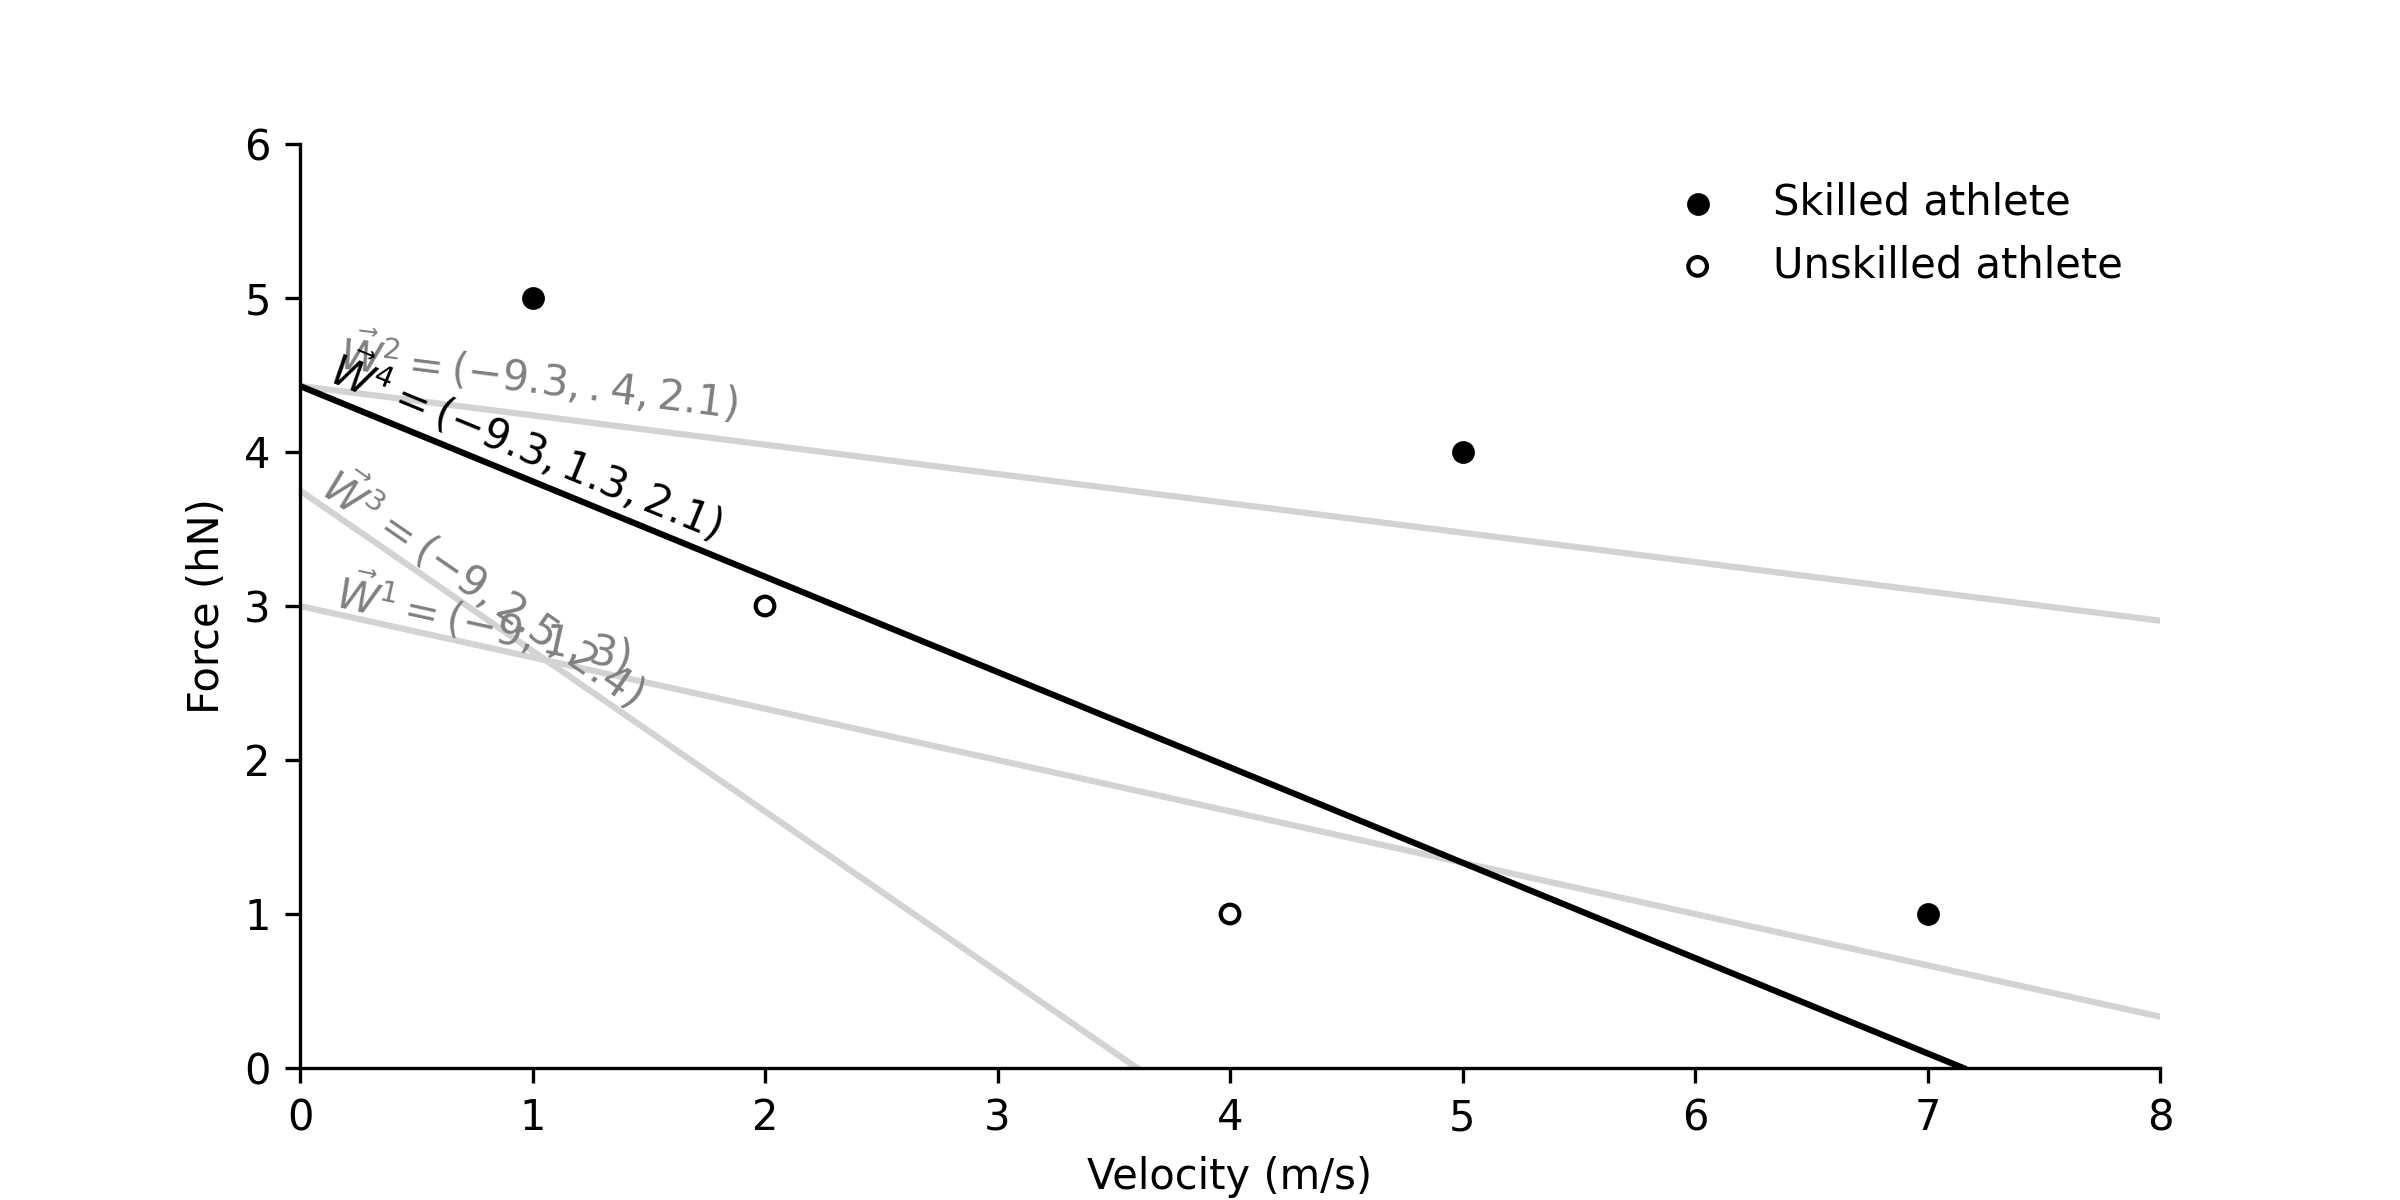
\includegraphics[width=\linewidth]{"../Chap2/Figures/Fig_perceptron.png"}
% 	\caption{Classification of athletes as "good" (black dot) or "bad" (circle) according to their Force-Velocity results. Weights are adjusted (grey lines), until the perceptron classifies athletes correctly (black line.)}
% 	\label{fig_perceptron}
% \end{figure}

% % En tikz
% \begin{figure}
% \centering
% \begin{tikzpicture}[x=0.5cm, y=0.5cm]
%     \draw[thick,->] (0,0) -- (0,6) node[anchor=south east] {Force (hN)};
%     \draw[thick,->] (0,0) -- (10,0) node[anchor=north west] {velocity (m/s)};
%     \foreach \x in {0,1,2,3,4,5,6,7,8,9}
%         \draw (\x,1pt) -- (\x,-1pt) node[anchor=north] {$\x$};
%     \foreach \y in {0,1,2,3,4,5}
%         \draw (1pt,\y) -- (-1pt,\y) node[anchor=east] {$\y$};
%     \foreach \Point in {(1,5), (5,4), (7,1)}{
%       \node at \Point {\textbullet};}
%     \foreach \Point in {(2,3), (4,1)}{
%       \node at \Point {$\circ$};}
%     % \node [green] at (5,4) {\textbullet};
%     % \node [red] at (2,3) {$\circ$};
%     \end{tikzpicture}
% \caption{Force-velocity results and classification.}
% \end{figure}

% % En matplotlib
% # Found on https://stackoverflow.com/questions/19907140/keeps-text-rotated-in-data-coordinate-system-after-resizing
% import matplotlib.pyplot as plt
% import numpy as np
% plt.rcParams.update({'font.size': 10})
% #import matplotlib.mathtext as mathtext
% import matplotlib.text as mtext
% import matplotlib.transforms as mtransforms

% class RotationAwareAnnotation(mtext.Annotation):
%     def __init__(self, s, xy, p, pa=None, ax=None, **kwargs):
%         self.ax = ax or plt.gca()
%         self.p = p
%         self.pa = pa
%         if not pa:
%             self.pa = xy
%         self.calc_angle_data()
%         kwargs.update(rotation_mode=kwargs.get("rotation_mode", "anchor"))
%         mtext.Annotation.__init__(self, s, xy, **kwargs)
%         self.set_transform(mtransforms.IdentityTransform())
%         if 'clip_on' in kwargs:
%             self.set_clip_path(self.ax.patch)
%         self.ax._add_text(self)

%     def calc_angle_data(self):
%         ang = np.arctan2(self.p[1]-self.pa[1], self.p[0]-self.pa[0])
%         self.angle_data = np.rad2deg(ang)

%     def _get_rotation(self):
%         return self.ax.transData.transform_angles(np.array((self.angle_data,)), 
%                             np.array([self.pa[0], self.pa[1]]).reshape((1, 2)))[0]

%     def _set_rotation(self, rotation):
%         pass

%     _rotation = property(_get_rotation, _set_rotation)

% plt.figure(figsize=(8, 4))
% plt.axis([0, 8, 0, 6])
% plt.gca().spines['top'].set_visible(False)
% plt.gca().spines['right'].set_visible(False)
% plt.gca().set_xlabel('Velocity (m/s)')
% plt.gca().set_ylabel('Force (hN)')

% velocity_good = [1,5,7]
% force_good = [5,4,1]
% velocity_bad = [2,4]
% force_bad = [3,1]
% plt.scatter(velocity_good, force_good, s=20, edgecolors='k', facecolors='k', label = "Skilled athlete")
% plt.scatter(velocity_bad, force_bad, s=20, edgecolors='k', facecolors='none', label="Unskilled athlete")
% plt.legend(frameon=False)

% # First lines with first weights, with dash greyed lines and label
% W=[-9,  1,  3]
% x1 = np.array( [0, -W[0]/W[1]] )
% x2 = np.array( [-W[0]/W[2], 0] )
% plt.plot(x1,x2, 'lightgrey')
% RotationAwareAnnotation(r'$\vec{W}^1=(-9,1,3)$', 
%       xy=(.15,3.3), p=[-W[0]/W[1],0], pa=[0,-W[0]/W[2]], ax=plt.gca(), xytext=(2,-1), textcoords="offset points", va="top", c='grey', bbox=dict(facecolor='None', edgecolor='None'))
    
% W=[-9.3, .4,  2.1]
% x1 = np.array( [0, -W[0]/W[1]] )
% x2 = np.array( [-W[0]/W[2], 0] )
% plt.plot(x1,x2, 'lightgrey')
% RotationAwareAnnotation(r'$\vec{W}^2=(-9.3, .4,  2.1)$', 
%       xy=(.15,4.85), p=[-W[0]/W[1],0], pa=[0,-W[0]/W[2]], ax=plt.gca(), xytext=(2,-1), textcoords="offset points", va="top", c='grey', bbox=dict(facecolor='None', edgecolor='None'))

% W=[-9,  2.5, 2.4]
% x1 = np.array( [0, -W[0]/W[1]] )
% x2 = np.array( [-W[0]/W[2], 0] )
% plt.plot(x1,x2, 'lightgrey')
% RotationAwareAnnotation(r'$\vec{W}^3=(-9,2.5,2.4)$', 
%     xy=(.15,4), p=[-W[0]/W[1],0], pa=[0,-W[0]/W[2]], ax=plt.gca(), xytext=(2,-1), textcoords="offset points", va="top", c='grey', bbox=dict(facecolor='None', edgecolor='None'))

% W=[-9.3,  1.3, 2.1]
% x1 = np.array( [0, -W[0]/W[1]] )
% x2 = np.array( [-W[0]/W[2], 0] )
% plt.plot(x1,x2, 'k')
% RotationAwareAnnotation(r'$\vec{W}^4=(-9.3,  1.3, 2.1)$', 
%       xy=(.15,4.75), p=[-W[0]/W[1],0], pa=[0,-W[0]/W[2]], ax=plt.gca(), xytext=(2,-1), textcoords="offset points", va="top", bbox=dict(facecolor='None', edgecolor='None'))

% plt.savefig(r'D:\softs\github_david\These_David_Pagnon\Thesis\Chap2\Figures\Fig_perceptron', dpi=300)
% plt.show()


%%%%%%%%%%%%%%%%%%%%%%%%%%%%%%%%%%%%%%%%%%%%%%%%%%%%%%%%%%%%%%%
% Figure linearly separable                                   %
%%%%%%%%%%%%%%%%%%%%%%%%%%%%%%%%%%%%%%%%%%%%%%%%%%%%%%%%%%%%%%%

% import matplotlib.pyplot as plt
% import numpy as np
% plt.rcParams.update({'font.size': 8})

% # Place dots on graph on click and record position
% # adapted from https://stackoverflow.com/a/41825214/12196632
% fig = plt.figure()
% ax = fig.add_subplot(111)
% ax.set_xlim([0, 10])
% ax.set_ylim([0, 10])

% def onclick(event):
%     print(f'{event.xdata}, {event.ydata}')
%     plt.plot(event.xdata, event.ydata, 'o')
%     fig.canvas.draw()
% cid = fig.canvas.mpl_connect('button_press_event', onclick)
% plt.show()


% # Plot examples of linearly and non-liearly separable data
% fig, axs = plt.subplots(1,4,figsize=(10,3))
% plt.rcParams.update({'font.size': 8})

% axs[0].scatter([1.31,4.11,3.22,1.61,5.30,7.52], [7.58,8.33,5.93,3.63,6.31,8.79],s=20, edgecolors='k', facecolors='k')
% axs[0].scatter([6.55,8.71,8.87,9.03,6.55,2.21,6.09], [0.65,0.65,3.22,6.33,4.33,1.46,2.93],s=20, edgecolors='k', facecolors='None')
% axs[0].plot([0,10],[1,10])
% axs[0].text(0.5,0.5,'(a)')

% axs[1].scatter([1.65,4.23,2.38,1.05,3.08,8.65,9.35,8.97,6.67, 7.19,3.00,2.00], [8.91,8.61,6.31,1.87, 0.25,0.63,4.85,8.12,0.63,8.55,2.00,4.00],s=20, edgecolors='k', facecolors='k')
% axs[1].scatter([4.90,4.86,6.17,5.62,5.99,5.58,7.18], [4.96,3.55,3.52,4.23,5.42,2.66,4.47],s=20, edgecolors='k', facecolors='None')
% t = np.linspace(0, 2*np.pi, 100)
% axs[1].plot(6+1.8*np.cos(t) , 4+2*np.sin(t),'-')
% axs[1].text(0.5,0.5,'(b)')

% axs[2].scatter([0.54,3.04,7.01,3.70,1.35,4.23,7.21,9.11,8.32], [7.90, 8.66,9.01,6.85,5.00,0.44,1.16,0.43,3.49],s=20, edgecolors='k', facecolors='k')
% axs[2].scatter([0.56,2.39,4.55,9.19,6.37,6.47,3.06,4.37,9.17,4.83], [1.79,2.68,4.95,8.66,6.33,4.14,0.97,3.60,6.63,1.84],s=20, edgecolors='k', facecolors='None')
% axs[2].plot([0,10],[2,10])
% axs[2].plot([3,10],[0,5], c='tab:blue')
% axs[2].text(0.5,0.5,'(c)')

% axs[3].scatter([1.67,3.08,6.81,9.23,6.67,2.06,4.96,5.62], [7.96,4.50,6.85,2.79,0.33,0.87,3.36,7.66],s=20, edgecolors='k', facecolors='k')
% axs[3].scatter([8.68,1.79,3.85,4.73,4.03,8.06,8.83,8.68], [6.52,3.85,2.41,5.03,8.09,2.92,0.49,8.93],s=20, edgecolors='k', facecolors='None')
% axs[3].text(5,3.5,'?',fontsize=70, **{'color':'tab:blue', 'fontfamily':'monospace'})
% axs[3].text(0.5,0.5,'(d)')

% for ax in axs:
%     ax.set_xlim([0, 10])
%     ax.set_ylim([0, 10])
%     ax.spines['top'].set_visible(False)
%     ax.spines['right'].set_visible(False)

% fig.savefig(r'D:\softs\github_david\These_David_Pagnon\Thesis\Chap2\Figures\Fig_linearly_sep', dpi=300)
% fig.show()


%%%%%%%%%%%%%%%%%%%%%%%%%%%%%%%%%%%%%%%%%%%%%%%%%%%%%%%%%%%%%%%
% Simple 3x3 line filter on image                             %
%%%%%%%%%%%%%%%%%%%%%%%%%%%%%%%%%%%%%%%%%%%%%%%%%%%%%%%%%%%%%%%

% # # Inspired from https://www.codingame.com/playgrounds/2524/basic-image-manipulation/filtering

% import cv2
% import numpy as np
% import os

% # Load image:
% dir_path = r'D:\softs\github_david\These_David_Pagnon\Thesis\Chap2\Figures'
% input_image = cv2.imread(os.path.join(dir_path,r"out_skewed.png"))
% width, height, _ = input_image.shape

% ## Calculate pixel intensity as the average of red, green and blue colors.
% intensity = [[sum(input_image[x, y]) / 3 for y in range(height)] for x in range(width)]

% # Line filter
% kernelx = [[-1, 0, 1],
%            [-2, 0, 2],
%            [-1, 0, 1]]
% # kernelx = [[-2,-1, 0, 1, 2],
% #            [-2,-1, 0, 1, 2],
% #            [-3,-2, 0, 2, 3],
% #            [-2,-1, 0, 1, 2],
% #            [-2,-1, 0, 1, 2]]

% # Create output image
% output_image = input_image.copy()

% # Compute convolution between intensity and kernels
% for x in range(1, width - 1):
%     for y in range(1, height - 1):
%         magx, magy = 0, 0
%         for a in range(3):
%             for b in range(3):
%                 xn = x + a - 1
%                 yn = y + b - 1
%                 magx += intensity[xn][yn] * kernelx[a][b]

%         # Draw in black and white the magnitude
%         output_image[x, y] = (magx, magx, magx)

% # Transform black pixels to transparent
% # alpha = np.sum(output_image, axis=-1) > 0  
% # alpha = np.uint8(alpha * 255)
% # output_image = np.dstack((output_image, alpha))

% # cv2.imshow('',output_image)
% cv2.imwrite(os.path.join(dir_path,r"out.png"), output_image)